

% a changed copy from the thesis

%\documentclass[a4paper,10pt,twocolumn]{article}
% use option draft to check for typesetting problems.
% similar to original word document

% don't use textheight... with koma-script
\documentclass[%draft,
%    a4paper,12pt, % 'Standard'
    11pt, % use explicit paper format for Java book format
%    b5paper,10pt, % B5 printout
    % use BCOR to compensate for the two-side margin!
%    a4paper,12pt,BCOR37pt,DIV15,
%    a4paper,12pt,BCOR40pt,DIV14,
%    b5paper,10pt,DIV12,
    headinclude, footexclude,
    twoside, % this produces strange margins!
    openright, % for new chapters
    cleardoubleempty,
% normalheadings - smaller chapter or smallheadings - too small
    % abstracton, % the author of koma-script argues against the title
    headsepline,
%    5headlines, % standard is 1.25 -- wirkt net!
    pointlessnumbers,
    ]{scrreprt}

%\usepackage{html}

% headings
\usepackage{scrpage2} % for headers
 \setkomafont{pagehead}{\scshape\small}
 \setkomafont{pagenumber}{\scshape\small}
 \automark[section]{chapter}
 \ohead[]{\pagemark}
 \chead[]{}
 \ihead[]{\headmark}
 \ofoot[]{} \cfoot[]{} \ifoot[]{}

%\tolerance=500 % to avoid lines sticking out into the margin
               % needed for 'high-performance' in Intro - contributions
\emergencystretch=2em
% or tol. to 500 and emerg. to 1em?
% pagebreak was ok with 500 and 1em
\interfootnotelinepenalty=10000


% use BCOR = (paperwidth-textwidth)/4
% A4: 210mm x 297mm
% B5: 176mm x 250mm
% Java book: 185mm x 232mm
% Engblom: 120x188 (without head)
% Java: 127x187 (without head)
% 1pt = 1/72.27 in = 0.351 mm


% for book
% 'Java-format' 526pt x 660pt (Ghostscript)
\setlength{\paperwidth}{185mm} \setlength{\paperheight}{232mm}
% use that BCOR setting with twoside to compensate the margin
\areaset[13.75mm]{130mm}{200mm} % Java book format

% for book to A4 conversion:
% Set the following sizes and export with
% 'Variable Page Size' in gs.
% Print with 'fit to paper' in Acrobat - results in 110%
% and an effective text area of 142x215
%\setlength{\paperwidth}{180mm} \setlength{\paperheight}{232mm}
%\areaset[12.5mm]{130mm}{200mm} % Java book format

% for two page printout in .pdf
%\setlength{\paperwidth}{134mm} \setlength{\paperheight}{206mm}
%\areaset[1mm]{130mm}{200mm} % Java book format


% use 10pt for code instead of 11pt - but I still would prefer Lucida Typewriter
%\newfont{\myttfont}{cmss10 scaled 1000}
%\newfont{\myttbfont}{cmssdc10 scaled 1000}
%
% This IS Lucida Typewriter
%\newfont{\myttfont}{plsr8r scaled 950}
%\newfont{\myttbfont}{plsb8r scaled 950}
%\newfont{\myttifont}{plsro8r scaled 950}
%%\newfont{\mytttextfont}{plsr8r}

% Lucida is perhaps available in the new Tex installation!!!!
% does not really work!!!
\newfont{\myttfont}{hlsrt8r scaled 950}
\newfont{\myttbfont}{hlsbt8r scaled 950}
\newfont{\myttifont}{hlsrot8r scaled 950}

% I used these .ttf for the official Thesis
%..\ttf2pt1 -e -b LucidaTypewriterRegular.ttf plsr8a
%..\ttf2pt1 -e -b LucidaTypewriterBold.ttf plsb8a
%..\ttf2pt1 -e -b LucidaTypewriterOblique.ttf plsro8a
%..\ttf2pt1 -e -b LucidaTypewriterBoldOblique.ttf plsbo8a

%\newcommand{\javatt}{\myttfont}
%\newcommand{\javattb}{\myttbfont}
%\newcommand{\javatti}{\myttifont}
%\newcommand{\javatext}{\myttfont}
%
%\newcommand{\picscale}{0.909}
%\newcommand{\excelwidth}{11cm}

% end book

% for B5
%\newfont{\javatt}{cmss10}
%\newfont{\javattb}{cmssdc10}
%\newcommand{\picscale}{0.833}
%\newcommand{\excelwidth}{10cm}



% for A4
% 12pt A4 scaled from book
%\areaset[17.05mm]{142mm}{219mm}
\newfont{\javatt}{cmss12}
\newfont{\javattb}{cmssdc10 scaled 1200}
% TODO find an italic
\newfont{\javatti}{cmss12}
\newcommand{\javatext}{\javatt}

\newcommand{\picscale}{1}
\newcommand{\excelwidth}{12cm}


% for chapter head without a number
% \renewcommand{\chaptermark}[1]{\def\myleftmark{#1}}
% \ihead{\myleftmark} \chead{} \ohead{{\rightmark}}

\setkomafont{captionlabel}{\sffamily\bfseries}



% Do I need this package?
\usepackage{float}

% is this a correction for the <> problem?
% \usepackage[T1]{fontenc}

\usepackage{pslatex} % -- times instead of computer modern
% pslatex should be replaced by this:
%\usepackage{mathptmx}
%\usepackage[scaled=.90]{helvet}
%\usepackage{courier}
% pslatex does not work with T1 encoding. <> Problem?


\usepackage{latexsym}
\usepackage{graphicx}
\usepackage{amsmath}
\usepackage{longtable}
\usepackage{booktabs}

% I would need Lucida Console!!!
%
%\newfont{\javatt}{pltt12} % lucida teletype, better than normal but with serifs
%\newfont{\javatt}{plss12} % lucida no serifes, but variable spacing
%\newfont{\javatt}{plss10 scaled 1200}
%\newfont{\javattb}{plssdc10 scaled 1200}
% cmss is NOT a tt font....


\usepackage{listings}
\lstset{language=Java,keywordstyle=,
basicstyle=\javatt,emphstyle=\javattb,commentstyle=\javatti,
showstringspaces=false,captionpos=b}

\usepackage{array}
\usepackage{dcolumn}
\newcommand{\cc}[1]{\multicolumn{1}{c}{#1}}
\newcolumntype{d}[1]{D{.}{.}{#1}}

% f�r die Umlaute in der Kurzfassung
% bekomme ich dadurch Probleme???
%\usepackage[ansinew]{inputenc}


\usepackage{capt-of}
\usepackage[colorlinks=true,linkcolor=black,citecolor=black]{hyperref}
%\usepackage{hyperref}

% ----------------------

%\usepackage{makeidx}
%\makeindex


\usepackage{import} % for subimport text and graphics from subdirectory
% does not work with latex2html!


\newcommand{\codefoot}{\textsf}
\newcommand{\code}[1]{{\javatext#1}} % for LaTeX
\newcommand{\cmd}[1]{{\texttt{#1}}}
\newcommand{\dirent}[1]{{\texttt{#1}}}
%\newcommand{\menuitem}[1]{\textsf{\textbf{#1}}}
\newcommand{\menuitem}[1]{\textsf{\textsl{#1}}}

% for flow.tex - part of index helper
\newcommand{\eei}[1]{%
\index{extension!\texttt{#1}}\texttt{#1}}

% JVs et al
%\newcommand{\ea}{et al.\xspace}
\newcommand{\ea}{et al.\ }

%\begin{htmlonly}
%\renewcommand{\code}[1]{{\texttt{#1}}} % for html2LaTeX
%\newcommand{\toprule}{\hline}
%\newcommand{\midrule}{\hline}
%\newcommand{\bottomrule}{\hline}
%\end{htmlonly}

% net wirklich notwendig -- h�ngt von code generierung ab
%\begin{htmlonly}
%\renewcommand{\javatt}{\texttt}
%\renewcommand{\javattb}{\texttt\bfseries}
%\end{htmlonly}

%\code{\hyphenchar\font=-1}

\newcommand{\mycomment}[1]{}

\newcommand{\instr}[6]{
    \begin{table}
        \begin{tabular}{ll}
            \emph{\large\textbf{#1}} & \\
            \\ \\
            \textbf{Operation} & #2 \\ \\
            \textbf{Opcode} & \texttt{#3} \\ \\
            \textbf{Dataflow} & \parbox[t]{9.5cm}{\(#4\)}\\ \\
            \textbf{JVM equivalent} & \parbox[t]{9.5cm}{\code{#5}} \\ \\
            \textbf{Description} & \parbox[t]{9.5cm}{#6}\\
        \end{tabular}
    \end{table}
}



\begin{document}

\title{JOP User Manual}
\author{Martin Schoeberl\\martin@jopdesign.com}
\maketitle \thispagestyle{empty}

%\input{intro/title}


%\input{intro/abstract}

\pagestyle{scrheadings} \pagenumbering{roman}

\tableofcontents \cleardoublepage
 \listoftables \newpage \listoffigures
 \newpage \lstlistoflistings \newpage

\chapter*{Foreword}

This book is about JOP, the Java Optimized Processor. JOP began as
research project for a PhD thesis. JOP has been used in several
industrial applications and, due to the fact that it is an
open-source project, has a growing user base. This book is written
for all of you who build this living community. The book is based to
some extent on the PhD thesis. For a long time the thesis, some
research papers, and the web site  have been the only available
documentation for JOP. A thesis is quite different to a user manual.
Its focus is on research results and implementation details are
usually omitted. This book fills the gap and provides inside into
the implementation of JOP and the accompanying Java virtual machine
(JVM). It also gives you an idea how to build an embedded real-time
system based on JOP.


\pagestyle{scrheadings} \pagenumbering{arabic}


%-----------------------------------------------------------------
% here we start to work
%-----------------------------------------------------------------

\chapter{Introduction}
\label{chap:intro}
%    

This handbook introduces a Java processor for embedded real-time
systems, in particular the design of a small processor for
resource-constrained devices with time-predictable execution of Java
programs. This Java processor is called JOP -- which stands for Java
Optimized Processor --, based on the assumption that a full native
implementation of all Java bytecode instructions is not a useful
approach.

\section{A Quick Tour on JOP}

In the following section we will give a quick overview on JOP and a
short description how to get JOP running within an FPGA. A detailed
description of the build process can be found in
Chapter~\ref{chap:build}.

JOP is the soft-core written in VHDL plus tools, a simplified Java
library (JDK), and some application examples. JOP is delivered in
source only. The source contains a set of VHDL files for the
processor core and Java files. The JOP sources are hosted at
Opencores\footnote{\url{http://www.opencores.org/projects.cgi/web/jop}}.


\subsection{Building JOP and Running ``Hello World"}

To build JOP you first have to download the source tree from
Opencores. A \emph{Makefile} (or an Ant file) contains all necessary
steps to build the tools, the processor, and the application.
Configuration of the FPGA and downloading the Java application is
also part of the Makefile.

In this description we assume the FPGA board Cycore (see
Appendix~\ref{appx:cycore}). This board is the default target for
the Makefile. The board has to be connected to the power supply and
to the PC via a ByteBlaster download cable and a serial cable.

The FPGA is configured via the ByteBlaster cable. The Java
application is downloaded after the FPGA configuration via the serial
cable. Besides the download the serial cable is also used as a
communication link between JOP and the PC. \code{System.out} and
\code{System.in} represent this serial link on JOP.

In order to build the whole system you need a Java
compiler\footnote{Download the Java SE Development Kit (JDK) from
\url{http://java.sun.com/javase/downloads/index.jsp}.} and an FPGA
compiler. In our case we use the free web edition of Quartus from
Altera\footnote{\url{http://www.altera.com/}}. As we use \cmd{make}
and the preprocessor from the GNU compiler collection,
Cygwin\footnote{\url{http://www.cygwin.com/}} should be installed
under Windows.

When all tools are setup correctly\footnote{Check at the command
prompt that \cmd{javac} is in the path.} a simple \cmd{make} should
build the tools, the processor, compile the ``Hello World" example,
configure the FPGA and download the application. The whole build
process will take a few minutes. After typing
\begin{verbatim}
    make
\end{verbatim}
you should see a lot of messages from the various tools. However,
the last lines should be actual messages received from JOP. It
should look similar to the following:
\begin{verbatim}
    JOP start
    ...
    V 20070831 - 60 MHz, 1024 KB RAM
    Hello World from JOP!

    JVM exit!
\end{verbatim}
Note that JOP prints some internal information, such as version and
memory size, at startup. After that, the message ``Hello World from
JOP!" can be seen. Our first program runs on JOP!

As a next step, locate the Hello World example in the source
tree\footnote{\dirent{.../jop/java/target/src/test/test/HelloWorld.java}}
and change the output message. The tools and the processor have been
built already. So we do not need to compile everything from scratch.
Use the following make target to just compile the Java application
and download the processor and the application:
\begin{verbatim}
    make japp
\end{verbatim}
The compile process should now be faster and the output similar to
before.

The Hello World application is the default target in the Makefile.
See Chapter~\ref{chap:build} for a description how this target can be
changed. In case you use a different FPGA board you can find
information on how to change the build process also in
Chapter~\ref{chap:build}.

\subsection{The Design Structure}

Browsing the source tree of JOP can give the impression that the
design is complex. However, the basic structure is not that complex.
The design consists of three entities:
\begin{enumerate}
    \item The processor JOP
    \item Supporting tools
    \item The Java library and application
\end{enumerate}

The different entities are also reflected during the configuration
and download process. The download is a two step process:
\begin{enumerate}
    \item Configuration of the FPGA: JOP is downloaded via a
    FPGA download cable (e.g.\ ByteBlaster on the PCs parallel
    port). After FPGA configuration the processor automatically starts and
    listens to the second channel (the serial line) for the software download.
    \item Java application download: the compiled and linked
    application is downloaded usually via a serial line. JOP stores
    the application in the main memory and starts execution at
    \code{main()} after the download.
\end{enumerate}

Further details of the source structure can be found in
Section~\ref{sec:directory}.

\section{A Short History}

The first version of JOP was created in 2000 based on the adaptation
of earlier processor designs created between 1995 and 2000. The first
version was written in Altera's proprietary AHDL language. The first
\emph{program} (3 bytecode instructions) ran on JOP on October 2,
2000. The first approach was a general purpose accumulator/register
machine with 16-bit instructions, 32-bit registers, and a pipeline
length of 3. It used the on-chip block memory to implement (somehow
unusual) 1024 registers.

The JVM was implemented in the assembler of that machine. That
concept was similar to the microcode in the current JOP version. The
decoding of the bytecode was performed by a long jump table. In the
best case (assuming a local, single cycle memory) a simple bytecode
(e.g.\ \code{iadd}) took 12 cycles for fetch and decode and
additional 11 cycles for execution.


A redesign followed in April 2001, now coded in VHDL. The version 2
of JOP introduced features to speed up the implementation of the JVM
with specific instructions for the stack access and a dedicated stack
pointer. The register file was reduced to 16 entries and the
instruction width reduced to 8 bits. The pipeline contained 5 stages
and special support for decoding bytecode instructions was added -- a
first version of the dynamic bytecode to microcode address
translation as it is used in the current version of JOP. The
enhancements within JOP2 resulted in the reduction of the execution
time for a simple bytecode to 3 cycles. A great enhancement compared
to the 23 cycles in JOP1.

The next redesign (JOP3) followed in June 2001. The challenge was to
execute simple bytecodes fully pipelined in a single cycle. The
microcode instruction set was changed to implement a stack machine
and the execution stage combined with the on-chip stack cache.
Microcode instructions where coded in 16 bit and the pipeline was
reduced to four stages. JOP3 is the basis of JOP as it is described
in this handbook. The later changes have not been so radical to call
them a redesign.

The first real-world application of JOP was in the project
\emph{Kippfahrleitung} (see Section~\ref{sec:app:kfl}). At the start
of the project (October 2001) JOP could only execute a single static
method stored in the on-chip memory. The project greatly pushed the
development of JOP. After successful deployment of the JOP-based
control system in the field, several projects followed (TeleAlarm,
Lift, the railway control system). The source of the commercial
applications is part of the JOP distribution. Some of these
applications are now used as a test bench for embedded Java
performance and to benchmark WCET analysis tools.

More details and the source code of
JOP1\footnote{\url{http://www.jopdesign.com/jop1.jsp}},
JOP2\footnote{\url{http://www.jopdesign.com/jop2.jsp}} and the first
JOP3\footnote{\url{http://www.jopdesign.com/jop3.jsp}} version are
available on the web site.


\section{JOP Features}

This book presents a hardware implementation of the Java virtual
machine (JVM), targeting small embedded systems with real-time
constraints. The processor is designed from the ground up for low
worst-case execution time (WCET) of bytecodes, in order to give
tasks low WCET values.

JOP is a stack computer with its own instruction set, called
microcode in this book. Java bytecodes are translated into microcode
instructions or sequences of microcode. The difference between the
JVM and JOP is best described as the following:
\begin{quote}
The JVM is a CISC stack architecture, whereas JOP is a RISC stack
architecture.
\end{quote}

JOP will help to increase the acceptance of Java for embedded
real-time systems. JOP is implemented as a soft-core in a field
programmable gate array (FPGA). Implementing a processor for
embedded systems in an FPGA gives a lot of flexibility for the
overall hardware design. The processor can easily be extended by
peripheral components inside the same chip. Therefore, it is
possible to customize the solution exactly to the needs of the
system.

JOP is designed from the ground up with time-predictable execution of
Java bytecode as a major design goal. All functional units, and
especially the interactions between them, are carefully designed to
avoid any time dependency between bytecodes. The architectural
features and highlights are:

\begin{itemize}

    \item The execution time for Java bytecodes can be exactly
        predicted in terms of the number of clock cycles. There
        is no mutual dependency between consecutive bytecodes.
        Therefore, no pipeline analysis -- with possible
        unbounded timing effects -- is necessary. These
        properties result in a simple processor model for the
        low-level WCET analysis.

    \item In order to fill the gap between processor speed and
        the memory access time, caches are mandatory. In
        Section~\ref{sec:cache}, a novel way to organize an
        instruction cache, as \emph{method cache}, is provided.
        The time predictable instruction cache caches whole
        methods. Only invoke and return instructions can result
        in a cache miss. All other instructions are guaranteed
        cache hits. This method cache is simple to analyze with
        respect to worst-case behavior and still provides a
        substantial performance gain.


Prefetch buffers or store buffers that can introduce unbounded
time dependencies between instructions are completely avoided in
the design. Even simple processors can contain an instruction
prefetch buffer that prohibits exact WCET values. The design of
the method cache and the translation unit avoids the variable
latency of a prefetch buffer.



    \item JOP is microprogrammed using a novel way of mapping
        bytecodes to microcode addresses. This mapping has
        minimum overheads, even for complex bytecodes. CISC Java
        bytecodes are dynamically translated to a RISC,
        stack-based instruction set (the microcode) that can be
        executed in a 3 stage pipeline.


The translation takes exactly one cycle per bytecode and is
therefore pipelined. Compared to other forms of dynamic code
translation, the translation does not add any variable latency to
the execution time and is therefore time predictable.

    \item The short pipeline (4 stages) results in short
        conditional branch delays and a hard-to-analyze branch
        prediction logic or a branch target buffer can be
        avoided. All microcode instructions are executed in
        constant time (one cycle). There are no stalls in the
        microcode pipeline. Loads and stores of object fields are
        handled explicitly. Interrupts are inserted in the
        translation stage as special bytecodes and are
        transparent to the microcode pipeline.


    \item A two-level stack cache, described in
        Section~\ref{sec:stack}, which fits in the embedded
        memory technologies of current FPGAs and ASICs, ensures
        the fast execution of basic instructions with minimum
        resource requirements.


The first level consists of the two topmost stack elements as
discrete registers. Those two registers are the basis of the
execution stage. The combination of the first level stack cache and
the execution unit does not need a write back stage or any
forwarding logic.


The second level provides fast and time predictable access to local
variables and the operand stack. Access to local variables is a
guaranteed hit and no pipeline stall can happen. Fill and spill of
the stack cache is subjected to microcode control and therefore
analyzable.


    \item
JOP is the smallest hardware implementation of the JVM available to
date. This fact enables usage of low-cost FPGAs in embedded systems.
The resource usage of JOP can be configured to trade size against
performance for different application domains.

Avoidance of hard-to-analyze architectural features results in
the very small design. Therefore, the available real estate can
be used for a chip multi-processor version of JOP as described in
Chapter~\ref{chap:cmp}.


    \item
JOP is actually in use in several real-world applications showing
that a Java based embedded system implemented in an FPGA is a viable
option. In Section~\ref{sec:applications} the usage of JOP in a
real-world application is described.

\end{itemize}

This Java processor architecture results in time predictable and
high-performance execution of real-time tasks in Java, without the
resource implications and unpredictability of a JIT-compiler.

\section{Is JOP the Solution for Your Problem?}

I had a lot of fun, and still have, developing and using JOP.
However, should you use JOP? JOP is a processor design intended as a
time predictable solution for hard real-time systems. If your
application or research focus is on those systems and you prefer Java
as programming language, JOP is the right choice. If you are
interested in larger, dynamic systems, JOP is the wrong choice. If
average performance is important for you and you do not care about
worst-case performance other solutions will probably do a better job.

\section{Outline of the Book}

Chapter~\ref{chap:build} gives a detailed introduction into the
design flow of JOP. It explains how the individual parts are compiled
and which files have to be changed when you want to extend JOP or
adapt it to a new hardware platform. The chapter is concluded by an
exercise to evaluate the different steps in the design flow.

Chapter~\ref{chap:java} provides background information on the Java
programming language, the execution environment, and the Java virtual
machine, for Java applications. If you are already familiar with Java
and the JVM, feel free to skip this chapter.

Standard Java is not suitable for the resource-constrained world of
embedded systems. Chapter~\ref{chap:rtjava} gives an overview of
various definitions in embedded Java and the real-time specification
of Java (RTSJ). It is an extended version of \cite{jop:rtjava} and
Chapter~4 of \cite{jop:thesis}.

Chapter~\ref{chap:arch} is the main chapter in which the
architecture of JOP is described. The motivation behind different
design decisions is given. A Java processor alone is not a complete
JVM. Chapter~\ref{chap:runtime} describes the runtime environment on
top of JOP, including the definition of a real-time profile for Java
and a framework for a user-defined scheduler in Java.



Garbage collection (GC) is an important part of the Java technology.
Even in real-time systems new real-time garbage collectors emerge.
In Chapter~\ref{chap:rtgc} the formulas to calculate the correct
scheduling of the GC thread are given and the implementation of the
real-time GC for JOP is explained.

In Chapter~\ref{chap:wcet} WCET analysis of the individual Java
bytecodes is performed. It is shown how these bytecode instruction
timings form the basis of WCET analysis of Java applications.

JOP uses a simple and efficient system-on-chip interconnection
called SimpCon to connect the memory controller and peripheral
devices to the processor pipeline. The definition of SimpCon and the
rationale behind the SimpCon specification is given in
Chapter~\ref{chap:simpcon}.

%Chapter~\ref{chap:ejip} sketches the implementation of an embedded
%TCP/IP stack called \code{ejip}.

In Chapter~\ref{chap:results}, JOP is evaluated with respect to size
and performance. This is followed by a description of some
commercial real-world applications of JOP.

Other solutions are presented in Chapter~\ref{chap:related}.
Different hardware solutions from both academia and industry for
accelerating Java in embedded systems are analyzed.

Finally, in Chapter~\ref{chap:conclusions}, the work is summarized
and the major contributions are presented. This chapter concludes
with directions for future research using JOP and real-time Java.

\section{Is JOP the Solution for Your Problem?}

\emph{TODO: move is to the correct place.}

I had a lot of fun, and still have, developing and using JOP, but
should you use JOP? JOP is a processor design intended as a time
predictable solution for hard real-time systems. If your application
or research focus is on those systems and you prefer Java as
programming language JOP is the right choice. If you are interested
in larger, dynamic systems JOP is the wrong choice. If average
performance is important for you and you do not care about
worst-case performance other solutions will probably do a better
job.


\section{Directory Structure}
\label{sec:directory}

The top-level directories of the distribution are:

\begin{description}
    \item[asm] Microcode source files. The microcode part of the JVM
    and test files.
    \item[bat] Old batch files - \emph{not used}
    \item[boards] Pictures and text for the Eclipse plugin
    \item[c\_src] Some utilities in C (e.g.\ \cmd{down.exe} and
    \cmd{e.exe}).
    \item[doc] \LaTeX sources for this handbook and short notes.
    \item[eclipse] Eclipse project files
    \item[ext] External VHDL and Verilog sources
    \item[java] All Java files
    \begin{description}
        \item[lib] External .jar files
        \item[pc] Tools on the PC
        \item[pcsim] High-level simulation on the PC
        \item[target] \emph{The} Java sources for JOP
        \item[tools] All Java tools
    \end{description}
    \item[jbc] FPGA configuration files for \cmd{jbi32.exe} (generated)
    \item[jopc] A C version of a JOP JVM simulation -- \emph{very} outdated
    \item[linux] Scripts to start a network and SLIP
    \item[modelsim] ModelSim simulation
    \item[pins] Pin definitions for FPGA boards
    \item[quartus] Quartus project files
    \item[rbf] FPGA configuration files for USBRunner (generated)
    \item[sopc] JOP as SoPC component and SRAM components
    \item[support] Stand-alone Flash programming for the Cycore board
    \item[ttf] FPGA configuration files for Flash programming (generated)
    \item[vhdl] The processor sources
    \begin{description}
        \item[altera] Altera specific components (PLL, RAM)
        \item[config] Cycore PLD sources
        \item[core] The processor core
        \item[fpu] The floating-point unit
        \item[memory] Main memory connections vi SimpCon
        \item[scio] IO components and configurations with SimpCon
        \item[simpcon] SimpCon bridges and arbiter
        \item[simulation] Memory and UART for ModelSim simulation
        \item[start] The VHDL version of \emph{hello world} -- a blinking
        LED
        \item[testbenches] no real content
        \item[top] Top-level and configuration (e.g.\ PLL setting) components
        \item[vga] A SimpCon VGA controller
        \item[wishbone] WISHBONE files -- \emph{not used?}
        \item[xilinx] Xilinx specific components (RAM)
    \end{description}
    \item[xilinx] Xilins project files
\end{description}

\subsection{The Java Sources for JOP}

The most important directory for all Java sources that run on JOP is
in \dirent{java/target}.

\begin{description}
    \item[dist] Generated files
    \begin{description}
        \item[bin] The linked application (\code{.jop})
        \item[classes] The class files
        \item[lib] The application class files in \code{classes.zip}
        -- input for \cmd{JOPizer}
    \end{description}
    \item[src] The source
    \item[wcet] Output from the WCET analyzer (generated)
\end{description}


\chapter{Introduction into the Design Flow}
\label{chap:build}

This section describes the design flow for JOP --- how to build the
Java processor and a Java application from scratch (the VHDL and
Java sources) and download the processor to an FPGA and the Java
application to the processor.


\section{Introduction}

JOP \cite{jop:thesis}, the Java optimized processor, is an
open-source development available for different targets (Altera and
Xilinx FPGAs and various types of FPGA boards). To support several
targets the design-flow gets a little bit complicated. There is a
\code{Makefile} available and when everything is set up correct a
simple
%
\begin{verbatim}
    make
\end{verbatim}
%
should build everything from the sources and download a \emph{Hello
World} example. However, to customize the \code{Makefile} for a
different target it is necessary to understand the complete design
flow. It should be noted that an
Ant\footnote{\url{http://ant.apache.org/}} based build process is
also available and will in the future substitute the \cmd{make}
based build.

\subsection{Tools}

All needed tools are freely available.
%
\begin{itemize}
    \item  \href{http://java.sun.com/javase/downloads/index.jsp}%
{Java SE Development Kit (JDK)}  Java compiler and runtime
    \item  \href{http://www.cygwin.com/}%
{Cygwin} GNU tools for Windows. Packages cvs, gcc and make are
needed
    \item  \href{https://www.altera.com/support/software/download/altera_design/quartus_we/dnl-quartus_we.jsp}%
{Quarts II Web Edition} VHDL synthesis, place and route for Altera
FPGAs
%    \item  \href{https://www.altera.com/support/software/download/programming/jam/dnl-byte_code_player.jsp}%
%{Jam STAPL Byte-Code Player} FPGA configuration in batch mode
%(\cmd{jbi32.exe})

\end{itemize}
%
The PATH variable should contain entries to the executables of all
packages (java and javac, Cygwin bin, Quartus executables and
jbi32). Check the PATH at the command prompt with:
%
\begin{verbatim}
    javac
    gcc
    make
    cvs
    quartus_map
\end{verbatim}
%
All the executables should be found and usually report their usage.

\subsection{Getting Started}

This sections shows a quick step-by-step build of JOP for the
Cyclone target in the minimal configuration. All directory paths are
given relative to the JOP root directory \dirent{jop}. The build
process is explained in more detail in one of the following
sections.

\subsubsection{Download the Source}

Create a working directory and download JOP from the
\url{www.opencores.org} CVS server:

\begin{verbatim}
 cvs -d :pserver:anonymous@cvs.opencores.org:/cvsroot/anonymous \
    -z9 co -P jop
\end{verbatim}

All sources are downloaded to a directory \dirent{jop}. For the
following command change to this directory. Create the needed
directories with:
\begin{verbatim}
    make directories
\end{verbatim}

\subsubsection{Tools}

The tools contain \cmd{Jopa} the microcode assembler, \cmd{JopSim} a
Java based simulation of JOP, and \cmd{JOPizer} the application
builder. The tools are built with following make command:

\begin{verbatim}
    make tools
\end{verbatim}

\subsubsection{Assemble the Microcode JVM, Compile the Processor}

The JVM configured to download the Java application from the serial
interface is built with:

\begin{verbatim}
    make jopser
\end{verbatim}

This command also invokes Quartus to build the processer. If you
want to build it within Quartus follow the following instructions:

\label{subsubsec:quartus}

Start Quartus II and open the project \code{jop.qpf} from directory
\dirent{quartus/cycmin} in Quartus with \menuitem{File -- Open
Project...}. Start the compiler and fitter with \menuitem{Processing
-- Start Compilation}. After successful compilation the FPGA is
configured with \menuitem{Tools -- Programmer} and \menuitem{Start}.

\subsubsection{Compiling and Downloading the Java Application}

A simple \emph{Hello World} application is the default application
in the Makefile. It is built and downloaded to JOP with:

\begin{verbatim}
    make japp
\end{verbatim}

The ``Hello World" message should be printed in the command window.

For a different application change the Makefile targets or override
the \code{make} variables at the command line. Following example
builds and runs some benchmarks on JOP:

\begin{verbatim}
    make japp -e P1=bench P2=jbe P3=DoAll
\end{verbatim}

The three variables \code{P1}, \code{P2}, and \code{P3} are a
shortcut to set the directory, the package name, and the main class
of the application.

\subsection{Xilinx Spartan-3 Starter Kit}

\index{Xilinx} The Xilinx tool chain is still not well supported by
the Makefile or the Ant design flow. Here a short list how to build
JOP for a Xilinx board:

\begin{verbatim}
    make tools
    cd asm
    jopser
    cd ..
\end{verbatim}


Now start the Xilinx IDE on the project file \code{jop.npl}. It will
be converted to a new (binary) \code{jop.ise} project. The
\code{.npl} project file is used as it is simple to edit (ASCII).

\begin{itemize}
    \item Generate JOP by double clicking 'Generate PROM, ACE, or JTAG File'
    \item Configure the FPGA according to the board type
\end{itemize}

The above is a one step build for the processor. The Java
application is built and downloaded by:

\begin{verbatim}
    make java_app
    make download
\end{verbatim}

Now your first Java program runs on JOP/Spartan-3!

\section{Booting JOP --- How Your Application Starts}

Basically this is a two step process: (a) configuration of the FPGA
and (b) downloading the Java application. There are different ways
to perform these steps.

\subsection{FPGA Configuration}

FPGAs are usually SRAM based and \emph{lose} their configuration
after power down. Therefore the configuration has to be loaded on
power up. For development the FPGA can be configured via a download
cable (with JTAG commands). This can be done within the IDEs from
Altera and Xilinx or with command line tools such as
\cmd{quartus\_pgm} or \cmd{jbi32}.

When the device shall boot automatically the configuration has to be
stored in non volatile memory such as Flash. Serial Flash is
directly supported by an FPGA to boot on power up. Another method is
to use a standard parallel Flash to store the configuration and
additional data (e.g. the Java application). A small PLD reads the
configuration data from the Flash and shifts it into the FPGA. This
method is used on the Cyclone and ACEX boards.

\subsection{Java Download}

\index{application!download} When the FPGA is configured the Java
application has to be downloaded into the main memory. This download
is performed in microcode as part of the JVM startup sequence. The
application is a \code{.jop} file generated by \cmd{JOPizer}. At the
moment there are three options:

\begin{description}
    \item[Serial line] JOP listens to the serial line and the data
    is written into the main memory. A simple echo protocol performs
    the flow control. The baud rate is usually 115kBaud.
    \item[USB] Similar to the serial line version, JOP listens to the
    parallel interface of the FTDI FT2232 USB chip. The FT2232
    performs the flow control on the USB level and the echo
    protocol is omitted.
    \item[Flash] For stand alone applications the Java program is
    copied from the Flash (relative Flash address 0, mapped Flash
    address is 0x80000\footnote{All addresses in JOP are counted in
    32-bit quantities. However, the Flash is connected only to the
    lower 8 bits of the data bus. Therefore a store of one word in
    the main memory needs four loads from the Flash.}) to the main
    memory (usually a 32-bit SRAM).
\end{description}


To select on method for downloading a customized version of the JVM
is generated and the complete processor has to be built. The
generation is performed by the C preprocessor (\cmd{gcc}) on
\code{jvm.asm}. The serial version is generated by default, the USB
or Flash version are generated by defining the preprocessor
variables \code{USB} or \code{FLASH}.

\paragraph{VHDL Simulation}

\index{simulation!VHDL}To speed up the VHDL simulation in ModelSim
there is a forth method where the Java application is loaded by the
test bench instead of JOP. This version is generated by defining
\code{SIMULATION}. The actual Java application is written by
\cmd{jop2dat} into a plain text file (\code{mem\_main.dat}) and read
by the simulation test bench into the simulated main memory.

There are four small batch-files in directory \dirent{asm} that
perform the JVM generation: \cmd{jopser}, \cmd{jopusb},
\cmd{jopflash}, and \cmd{jopsim}.

\subsection{Combinations}

Theoretically all variants to configure the FPGA can be combined
with all variation to download the Java application. However, only
two combinations are useful:

\begin{enumerate}
    \item For VHDL or Java development configure the FPGA
    via the download cable and download the Java application
    via the serial line or USB.
    \item For a stand-alone application load the configuration and
    the Java program from the Flash.
\end{enumerate}



\section{The Design Flow}

This section describes the design flow to build JOP in greater
detail.

\subsection{Tools}

There are a few tools necessary to build and download JOP to the
FPGA boards. Most of them are written in Java. Only the tools that
access the serial line are written in C\footnote{The Java JDK still
comes without the javax.comm package and getting this optional
package correctly installed is not that easy.}.

\subsubsection{Downloading}

These little programs are already compiled and the binaries are
checked in into the CVS. The sources can be found in directory
\dirent{c\_src}.

\begin{description}
    \item[\eei{down.exe}] The workhorse to download Java programs. The
    mandatory argument is the COM-port. Optional switch \code{-e}
    keeps the program running after the download and echoes the
    characters from the serial line (\code{System.out} in JOP) to
    stdout. Switch \code{-usb} disables the echo protocol to speed up the
    download over USB.
    \item[\eei{e.exe}] Echo the characters from the serial line to stdout.
    Parameter is the COM-port.
    \item[\eei{amd.exe}] An utility to send data over the serial line to program
    the on-board Flash. The complementary Java program
    \code{util.Amd} must be running on JOP.
    \item[\eei{USBRunner.exe}] Download the FPGA configuration via
    USB with the FTDI2232C chip (dpsio board).
\end{description}

\subsubsection{Generation of Files}

These tools are written in Java and are delivered in source form.
The source can be found under \dirent{java/tools/src} and the class
files are in \code{jop-tools.jar} in directory
\dirent{java/tools/dist/lib}.

\begin{description}
    \item[\eei{Jopa}] The JOP assembler. Assembles the microcoded
    JVM and produces on-chip memory initialization files and VHDL
    files.
    \item[\eei{BlockGen}] converts Alter memory initialization files
    to VHDL files for a Xilinx FPGA.
    \item[\eei{JOPizer}] links a Java application and converts the
    class information to the format that JOP expects (a \code{.jop} file).
    \cmd{JOPizer} uses the bytecode engineering library\footnote{\url{http://jakarta.apache.org/bcel/}} (BCEL).

\end{description}

\subsubsection{Simulation}

\index{simulation!JopSim}
\begin{description}
    \item[\eei{JopSim}] reads a \code{.jop} file and executes it in
    a debug JVM written in Java. Command line option
    \code{-Dlog="true"} prints a log entry for each executed JVM
    bytecode.
    \item[\eei{pcsim}] simulates the BaseIO expansion board for Java
    debugging on a PC (using the JVM on the PC).
\end{description}

\subsection{Targets}

JOP has been successfully ported to several different FPGAs and
boards. The main distribution contains the ports for the FPGAs:

\begin{itemize}
    \item Altera Acex 1K30 or 1K50
    \item Altera Cyclone EP1C6 or EP1C12
    \item Xilinx Spartan-3
    \item Altera Cyclone-II (Altera DE2 board)
    \item Xilinx Virtex-4 (ML40x board)
    \item Xilinx Spartan-3E (Digilent Nexys 2 board)
\end{itemize}

For an actual list of the supported FPGA boards see the list at the
web site. Besides the ports to different FPGAs there are ports to
different boards.

\subsubsection{ACEX EP1K50C144 Jopcore}

This board was one of the first targets (besides the KFL project)
for JOP and the design files of the board are now available as
open-source from
\url{http://www.opencores.org/projects.cgi/web/acxbrd/overview}. As
the FPGA is a little bit dated the latest features of JOP (e.g. the
enhancements in the method cache) are not available in the Acex
port. Use \code{jop\_20040913\_v37\_web.zip} from the archive
section. Two Quartus projects for this board are available:
\code{acxmin}, a minimum configuration containing only a serial
interface, and \code{acxtal}, a configuration for the \emph{baseio}
extension board. The ACEX specific files are \code{jopacx.vhd} and
\code{mem.vhd}.

\subsubsection{Cyclone EP1C6/12}

This board is pin-compatible to the ACEX board and comes in two
versions: with an Cyclone EP1C6 or EP1C12. The board contains:

\begin{itemize}
    \item Altera Cyclone EP1C6Q240 or EP1C12Q240 FPGA (see data sheet)
    \item 1MB fast SRAM
    \item 512KB Flash (for FPGA configuration and program code)
    \item 32MB NAND Flash
    \item ByteBlasterMV port
    \item Watchdog with LED
    \item EPM7064 PLD to configure the FPGA from the Flash (on watchdog reset)
    \item Voltage regulator (1V5)
    \item Crystal clock (20 MHz) at the PLL input (up to 640 MHz internal)
    \item Serial interface (MAX3232)
    \item 56 general purpose IO pins
\end{itemize}

The Cyclone specific files are \code{jopcyc.vhd} or \code{jopcyc12}
and \code{mem32.vhd}. This FPGA board is designed as a module to be
integrated with an application specific IO-board. There exist
following IO-boards:
%
\begin{description}
    \item[simpexp] A simple bread board with a voltage regulator and
    a SUBD connector for the serial line
    \item[baseio] A board with Ethernet connection and EMC protected
    digital IO and analog input
    \item[bg263] Interface to a GPS receiver, a GPRS modem, keyboard
    and a display for a railway application
    \item[lego] Interface to the sensors and motors of the LEGO
    Mindstorms. This board is a substitute for the LEGO RCX.
    \item[dspio] Developed at the University of Technology Vienna, Austria for
    digital signal processing related work. All design files for this
    board are open-source.
\end{description}
%
Table~\ref{tab:cycio} lists the related VHDL files and Quartus
project directories for each IO board.

\begin{table}
    \centering

    \begin{tabular}{lll}
        \toprule
        IO board & Quartus & IO top level \\
        \midrule
        simpexp  & \dirent{cycmin} & \code{scio\_min.vhd} \\
        baseio  & \dirent{cycbaseio} & \code{scio\_baseio.vhd} \\
        bg263  & \dirent{cybg} & \code{scio\_bg.vhd} \\
        lego  & \dirent{cyclego} & \code{scio\_lego.vhd} \\
        dspio  & \dirent{dspio} & \code{scio\_dspio.vhd} \\
        \bottomrule

    \end{tabular}
    \caption{Quartus project directories and VHDL files for the different IO boards}
    \label{tab:cycio}

\end{table}


\subsubsection{Xilinx Spartan-3}

\index{Xilinx} The Spartan-3 specific files are \code{jop\_xs3.vhd}
and \code{mem\_xs3.vhd} for the Xilinx Spartan-3 Starter Kit and
\code{jop\_trenz.vhd} and \code{mem\_trenz.vhd} for the Trenz
Retrocomputing board.


\section{Eclipse}

In folder \dirent{eclipse} there are several Eclipse projects that
you can import into your Eclipse workspace. All projects use the
Eclipse path variable\footnote{Eclipse (path) variables are
workspace specific.} \code{JOP\_HOME} that has to point to the root
directory of the JOP sources. Under \menuitem{Window --
Preferences...} select \menuitem{General -- Workspace -- Linked
Resources} and create the path variable \code{JOP\_HOME} with
\menuitem{New...}.

Import the projects with \menuitem{File -- Import..} and
\menuitem{Existing Projects into Workspace}. Select as root
directory \dirent{.../jop/eclipse}, select the projects you want to
import and press \menuitem{Finish}. Table~\ref{tab:eclipse} shows
all available projects.

\begin{table}
    \centering

    \begin{tabular}{ll}
        \toprule
        Project & Content \\
        \midrule
        \dirent{jop} & The target sources \\
        \dirent{joptools} & Tools such as \code{Jopa}, \code{JopSim}, and \code{JOPizer} \\
        \dirent{pc} & Some PC utilities (e.g.\ Flash programming via UDP/IP) \\
        \dirent{pcsim} & Simulation of the basio hardware on the PC \\
        \bottomrule

    \end{tabular}
    \caption{Eclipse projects}
    \label{tab:eclipse}

\end{table}

Add the libraries from \dirent{.../jop/java/lib} (as external
archives) to the build path of the project
\dirent{joptools}\footnote{Eclipse can't use path variables for
external .jar files -- annoying}. If you prefer your workspace to be
not within the JOP directory tree just copy the content of
\dirent{.../jop/eclipse} to your Eclipse workspace and import the
projects from there.

\section{Simulation}

This section contains the information you need to get a simulation
of JOP running. There are two ways to simulate JOP:
%
{\samepage
\begin{itemize}
    \item High-level JVM simulation with \cmd{JopSim}
    \item VHDL simulation (e.g. with ModelSim)
\end{itemize}
}
%
This section is about running a VHDL simulation with ModelSim. All
simulation files are vendor independent and should run on any
versions of ModelSim or a different VHDL simulator. You can simulate
JOP even with the free ModelSim XE II Starter Xilinx version.

\subsection{Background Information}

\index{simulation!VHDL} To simulate JOP, or any other processor
design, in a vendor neutral way models of the internal memories
(block RAM) and the external main memory are necessary. Beside this,
only a simple clock driver is necessary. To speed-up the simulation a
little bit a simulation of the uart output, which is used for
\code{System.out.print()}, is also part of the package.

Table~\ref{tab:simfiles} lists the simulation files for JOP and the
programs that generates the initialization data. The non-generated
VHDL files can be found in directory \dirent{vhdl/simulation}.
%
\begin{table}
\small
    \centering

    \begin{tabular}{llll}
        \toprule
        VHDL file & Function & Initialization file & Generator \\
        \midrule
        \code{sim\_jop\_types\_100.vhd} & JOP constant definitions & - & - \\
        \code{sim\_rom.vhd} & JVM microcode ROM & \code{mem\_rom.dat} & \cmd{Jopa} \\
        \code{sim\_ram.vhd} & Stack RAM & \code{mem\_ram.dat} & \cmd{Jopa} \\
        \code{sim\_jbc.vhd} & Bytecode memory (cache) & - & - \\
        \code{sim\_memory.vhd} & Main memory & \code{mem\_main.dat} & \cmd{jop2dat} \\
        \code{sim\_pll.vhd} & A dummy entity for the PLL & - & - \\
        \code{sim\_uart.vhd} & Print characters to stdio & - & - \\
        \bottomrule

    \end{tabular}
    \caption{Simulation specific VHDL files}
    \label{tab:simfiles}

\end{table}
%
The needed VHDL files and the compile order can be found in
\code{sim.bat} under \dirent{modelsim}.


The actual version of JOP contains all necessary files to run a
simulation with ModelSim. In directory \dirent{vhdl/simulation} you
will find:
%
\begin{itemize}
    \item A test bench: \code{tb\_jop.vhd} with a serial receiver to
    print out the messages from JOP during the simulation
    \item Simulation versions of all memory components (vendor neutral)
    \item Simulation of the main memory
\end{itemize}
%
\cmd{Jopa} generates various \code{mem\_xxx.dat} files that are read
by the simulation. The JVM that is generated with \code{jopsim.bat}
assumes that the Java application is preloaded in the main memory.
\cmd{jop2dat} generates a memory initialization file from the Java
application file (\code{MainClass.jop}) that is read by the
simulation of the main memory (\code{sim\_memory.vhd}).

In directory \dirent{modelsim} you will find a small batch file
(\cmd{sim.bat}) that compiles JOP and the test bench in the correct
order and starts ModelSim. The whole simulation process (including
generation of the correct microcode) is started with:

\begin{verbatim}
    make sim
\end{verbatim}

After a few seconds you should see the startup message from JOP
printed in ModelSims command window.

\section{Files Types You Might Encounter}

As there are various tools involved in the complete build process,
you will find files with various extensions. The following list
explains the file types you might encounter when changing and
building JOP.

The following files are the \emph{source} files:

\begin{description}

\item[\eei{.vhd}] VHDL files describe the hardware part and are
compiled with either Quartus or Xilinx ISE. Simulation in ModelSim
is also based on VHDL files.
\item[\eei{.v}] Verilog HDL. Another hardware description language.
Used more in the US.

\item[\eei{.java}] Java --- the language that runs native on JOP.

\item[\eei{.c}] There are still some tools written in C.

\item[\eei{.asm}] JOP microcode. The JVM is written in this stack
oriented assembler. Files are assembled with \cmd{Jopa}. The result
are VHDL files, \code{.mif} files, and \code{.dat} files for
ModelSim.

\item[\eei{.bat}] Usage of these DOS batch files still prohibit
running the JOP build under Unix. However, these files get less used
as the \code{Makefile} progresses.

\item[\eei{.xml}] Project files for Ant. Ant is an attractive
substitution to \cmd{make}. Future distributions on JOP will be
\cmd{ant} based.

\end{description}


Quartus II and Xilinx ISE need configuration files that describe
your project. All files are usually ASCII text files.

\begin{description}

\item[\eei{.qpf}] Quartus II Project File. Contains almost no
information.
\item[\eei{.qsf}] Quartus II Settings File defines the project. VHDL
files that make up your project are listed. Constraints such as pin
assignments and timing constraints set here.
\item[\eei{.cdf}] Chain Description File. This file
stores device name, device order, and programming file name
information for the programmer.
\item[\eei{.tcl}] Tool Command Language. Can be used in Quartus to
automate parts of the design flow (e.g. pin assignment).

\item[\eei{.npl}] Xilinx ISE project. VHDL
files that make up your project are listed. The actual version of
Xilinx ISE converts this project file to a new format that is not in
ASCII anymore. Very annoying.
\item[\eei{.ucf}] Xilinx Foundation User Constraint File. Constraints
such as pin assignments and timing constraints set here.

\end{description}

\cmd{javac} and \cmd{jar} produce following file types from the Java
sources:

\begin{description}

\item[\eei{.class}] A class file contains the bytecodes, a symbol table and other
ancillary information and is executed by the JVM.

\item[\eei{.jar}] The Java Archive file format enables you to bundle multiple files
into a single archive file. Typically a \code{.jar} file contains
the class files and auxiliary resources. A \code{.jar} file is
essentially a zip file that contains an optional \dirent{META-INF}
directory.

\end{description}

The following files are generated by the various tools from the
source files:

\begin{description}

\item[\eei{.jop}] The file makes up the linked Java application that
runns on JOP. It is generated by \cmd{JOPizer} and can be either
downloaded (serial line or USB) or stored in the Flash (or used by
the simulation with \cmd{JopSim} or ModelSim)

\item[\eei{.mif}] Memory Initialization File. Defines the initial
content of on-chip block memories for Altera devices.

\item[\eei{.dat}] memory initialization files for the simulation
with ModelSim.

\item[\eei{.sof}] SRAM Output File. Configuration file for Altera
devices. Used by the Quartus programmer or by \cmd{quartus\_pgm}.
Can be converted to various (or too many) different format. Some are
listed below.

\item[\eei{.pof}] Programmer Object File. Configuration for Altera
devices. Used for the Flash loader PLDs.

\item[\eei{.jbc}] JamTM STAPL Byte Code 2.0. Configuration for Altera
devices. Input file for \cmd{jbi32}.

\item[\eei{.ttf}] Tabular Text File. Configuration for Altera
devices. Used by flash programming utilities (\cmd{amd} and
\cmd{udp.Flash} to store the FPGA configuration in the boards Flash.

\item[\eei{.rbf}] Raw Binary File. Configuration for Altera
devices. Used by the USB download utility (\cmd{USBRunner}) to
configure the dspio board via the USB connection.

\item[\eei{.bit}] Bitstream File. Configuration file for Xilinx
devices.

\end{description}

\section{Porting JOP}

Porting JOP to a different FPGA platform or board usually consists
of adapting pin definitions and selection of the correct memory
interface. Memory interfaces for the SimpCon interconnect can be
found in directory \dirent{vhdl/memory}.

\subsection{Test Utilities}

To verify that the port of JOP is successful there are some small
test programs in \dirent{asm/src}. To run the JVM on JOP the
microcode \code{jvm.asm} is assembled and will be stored in an
on-chip ROM. The Java application will than be loaded by the first
microcode instructions in \code{jvm.asm} into an external memory.
However, to verify that JOP and the serial line are working correct
it is possible to run small test programs directly in microcode.

One test program (\code{blink.asm}) does not need the main memory
and is a first test step before testing the possible changed memory
interface. \code{testmon.asm} can be used to debug the main memory
interface. Both test programs can be built with the \cmd{make}
targets \cmd{jop\_blink\-test} and \cmd{jop\_testmon}.

\subsubsection{Blinking LED and UART output}

In directory \dirent{asm} the blink test program is built with:
%
\begin{verbatim}
    build blink
\end{verbatim}
%
Compile and download the FPGA configuration as described in
Section~\ref{subsubsec:quartus}. After download the watchdog LED
should blink and the FPGA will print out 0 and 1 on the serial line.
Use a terminal program or the utility \cmd{e.exe} to check the
output from the serial line.

\subsubsection{Test Monitor}

In directory \dirent{asm} the test monitor is built with:
%
\begin{verbatim}
    build testmon
\end{verbatim}
%
Start a terminal program (e.g. HyperTerm) to communicate with the
monitor program. Compile and download the FPGA configuration as
described in Section~\ref{subsubsec:quartus}.

After download the program prints the content of the memory at
address 0. The program understands following \emph{commands}:

\begin{itemize}
    \item A single CR reads the memory at the current addres
    and prints out the address and memory content
    \item \code{addr=val;} writes $val$ into the memory location at
    address $addr$
\end{itemize}

One tip: Take care that your terminal program does not send a LF
after the CR.


\section{Extending JOP}

JOP is a soft-core processor and customizing it for an application
is an interesting opportunity.

\subsection{Native Methods}

\index{native method} The \emph{native} language of JOP is microcode.
A native method is implemented in JOP microcode. The interface to
this native method is through a \emph{special} bytecode. The mapping
between native methods and the special bytecode is performed by
\code{JOPizer}.

When adding a new (\emph{special}) bytecode to JOP following files
have to be changed:
\begin{enumerate}
    \item \code{jvm.asm} implementation
    \item \code{Native.java} method signature
    \item \code{JopInstr.java} mapping of the signature to the name
    \item \code{JopSim.java} simulation of the bytecode
    \item \code{JVM.java} (just rename the method name)
    \item \code{Startup.java} only when needed in a class initializer
    \item \code{WCETInstruction.java} timing information
\end{enumerate}

First implement the native code in \code{JopSim.java} for easy
debugging. The \emph{real} microcode is added in \code{jvm.asm} with
a label for the special byctecode. The naming convention is
\code{jopsys\_name}. In \code{Native.java} provide a method
signature for the native method and enter the mapping between this
signature and the name in \code{jvm.asm} and in
\code{JopInstr.java}. Provide the execution time in
\code{WCETInstruction.java} for the WCET analysis.

The native method is accessed by the method provided in
\code{Native.java}. There is no calling overhead involved in the
mechanism. The \emph{native} method gets substituted by
\cmd{JOPizer} with a \emph{special} bytecode.

\subsection{A new Peripheral Device}


Creation of a new peripheral devices involves some VHDL coding.
However, there are several examples in \dirent{jop/vhdl/scio}
available.


All peripheral components in JOP are connected with the SimpCon
\cite{simpcon} interface. For a device that implements the Wishbone
\cite{soc:wishbone} bus, a SimpCon-Wishbone bridge
(\code{sc2wb.vhd}) is available (e.g.\ it is used to connect the
AC97 interface in the \code{dspio} project).

For an easy start use an existing example and change it to your
needs. Take a look into \code{sc\_test\_slave.vhd}. All peripheral
components (SimpCon slaves) are connected in one module usually
named \code{scio\_xxx.vhd}. Browse the examples and copy one that
best fits your needs. In this module the address of your peripheral
device is defined (e.g. 0x10 for the primary UART). This IO address
is mapped to a negative memory address for JOP. That means
0xffffff80 is added as a base to the IO address.

By convention this address mapping is defined in
\code{com.jopdesign.sys.Const}. Here is the UART example:

\begin{verbatim}
    // use negative base address for fast constant load
    // with bipush
    public static final int IO_BASE = 0xffffff80;
    ...
    public static final int IO_STATUS = IO_BASE+0x10;
    public static final int IO_UART = IO_BASE+0x10+1;
\end{verbatim}

The IO devices are accessed from Java by
\emph{native}\footnote{These are not real functions and are
substituted by special bytecodes on application building with
JOPizer.} functions: \code{Native.rdMem()} and \code{Native.wrMem()}
in pacakge \code{com.jopdesign.sys}. Again an example with the UART:

\begin{verbatim}
    // busy wait on free tx buffer
    // no wait on an open serial line, just wait
    // on the baud rate
    while ((Native.rdMem(Const.IO_STATUS)&1)==0) {
        ;
    }
    Native.wrMem(c, Const.IO_UART);
\end{verbatim}

Best practise is to create a new IO configuration
\code{scio\_xxx.vhdl} and a new Quartus project for this
configuration. This avoids the mixup of the changes with a new
version of JOP. For the new Quartus project only the three files
\code{jop.cdf}, \code{jop.qpf}, and \code{jop.qsf} have to be copied
in a new directory under \dirent{quartus}. This new directory is the
project name that has to be set in the Makefile:

\begin{verbatim}
    QPROJ=yourproject
\end{verbatim}

The new VHDL module and the \code{scio\_xxx.vhdl} are added in
\code{jop.qsf}. This file is a plain ASCII file and can be edit with
a standard editor or within Quartus.

\subsection{A Customized Instruction}

A customized instruction can be simply added by implementing it in
microcode and map it to a native function as described before. If
you want to include a hardware module that implements this
instruction a new microinstruction has to be introduced. Besides
mapping this instruction to a native method the instruction has also
be added to the microcode assembler \cmd{Jopa}.

\subsection{Dependencies}

Changes to central (data) structures needs an update in several
files.

\subsubsection{Changing the Class Format}

\begin{itemize}
    \item JOPizer: CLS\_HEAD, dump()
    \item GC.java uses CLASS\_HEADR
    \item JMV.java uses CLASS\_HEADR + offset (checkcast, instanceof)
\end{itemize}

\subsubsection{Stack Size}

\begin{itemize}
    \item \code{ram\_width} in \code{jop\_config\_xx.vhd}
    \item \code{STACK\_SIZE} in \code{com.jopdesign.sys.Const}
    \item \code{RAM\_LEN} in \code{com.jopdesign.sys.Jopa}
\end{itemize}

\section{Acknowledgments}

Ed Anuff wrote \code{testmon.asm} to perform a memory interface test
and \code{BlockGen.java} to convert Altera \code{.mif} files to
Xilinx memory blocks. \code{BlockGen.java} was the key tool to port
JOP to Xilinx FPGAs in general and the Spartan-3 more specific.
Flavius Gruian wrote the initial version of \cmd{JOPizer} to
generate the \code{.jop} file from the application classes.
\cmd{JOPizer} is based on the open source BCEL and is a substitute
to the former used \code{JavaCodeCompact} from Sun.

\section{Information on the Web}

Further information on JOP and the build process can be found in the
Internet at following places:

\begin{itemize}
    \item \url{http://www.jopdesign.com/} is the main web site for
    JOP
    \item \url{http://www.jopwiki.com/} is a Wiki that can be freely
    edited by JOP users.
    \item \url{http://tech.groups.yahoo.com/group/java-processor/}
    hosts a mail list for discussions on Java processors in general
    and mostly on JOP related topics
\end{itemize}

%\section{Notes}
%
%TODO:
%
%\begin{itemize}
%    \item pcsim
%    \item JopSim
%\end{itemize}
%Formating ideas -- see Latax intro p 27
%\url{http://www.ctan.org/tex-archive/info/lshort/english/lshort.pdf}\\




%\printindex
%\pagestyle{empty}
%\chaptermark{} % remove chapter mark in the heading, but it does it on the
               % last page too!
\bibliographystyle{plain}
%\bibliographystyle{plnnolow} % changed plain.bst to keep upper case in titles
\bibliography{../bib/all}

%\def\rightmark{} % remove section part in the heading
\appendix
% \ihead{\leftmark} % use chapter (=\leftmark) on both pages in the appendix

%\chapter{Publications}
%    % This is a copy from /usr/doc

\begin{itemize}

\subsubsection*{2003}

\item Martin Schoeberl.
 Using a {J}ava Optimized Processor in a Real World Application.
 In {\em Proceedings of the First Workshop on Intelligent Solutions in
  Embedded Systems (WISES 2003)}, pages 165--176, Austria, Vienna, June 2003.

\item Martin Schoeberl.
 Design Decisions for a {J}ava Processor.
 In {\em Tagungsband Austrochip 2003}, pages 115--118, Linz, Austria,
  October 2003.

\item Martin Schoeberl.
 {JOP}: {A} {J}ava Optimized Processor.
 In R.~Meersman, Z.~Tari, and D.~Schmidt, editors, {\em On the Move to
  Meaningful Internet Systems 2003: Workshop on {J}ava Technologies for
  Real-Time and Embedded Systems (JTRES 2003)}, volume 2889 of {\em Lecture
  Notes in Computer Science}, pages 346--359, Catania, Italy, November 2003.
  Springer.

\subsubsection*{2004}

\item Martin Schoeberl.
 Restrictions of {J}ava for Embedded Real-Time Systems.
 In {\em Proceedings of the 7th IEEE International Symposium on
  Object-Oriented Real-Time Distributed Computing (ISORC 2004)}, pages
  93--100, Vienna, Austria, May 2004.

\item Martin Schoeberl.
 Design Rationale of a Processor Architecture for Predictable
  Real-Time Execution of {J}ava Programs.
 In {\em Proceedings of the 10th International Conference on
  Real-Time and Embedded Computing Systems and Applications (RTCSA 2004)},
  Gothenburg, Sweden, August 2004.

\item Martin Schoeberl.
 Real-Time Scheduling on a {J}ava Processor.
 In {\em Proceedings of the 10th International Conference on
  Real-Time and Embedded Computing Systems and Applications (RTCSA 2004)},
  Gothenburg, Sweden, August 2004.

\item Martin Schoeberl.
 {J}ava Technology in an {FPGA}.
 In {\em Proceedings of the International Conference on
  Field-Programmable Logic and its applications (FPL 2004)}, Antwerp, Belgium,
  August 2004.

\item Martin Schoeberl.
 A Time Predictable Instruction Cache for a Java Processor.
 In Robert Meersman, Zahir Tari, and Angelo Corsario, editors, {\em On
  the Move to Meaningful Internet Systems 2004: Workshop on {J}ava Technologies
  for Real-Time and Embedded Systems (JTRES 2004)}, volume 3292 of {\em
  Lecture Notes in Computer Science}, pages 371--382, Agia Napa, Cyprus,
  October 2004. Springer.

\subsubsection*{2005}

\item Flavius Gruian, Per Andersson, Krzysztof Kuchcinski, and Martin Schoeberl.
 Automatic generation of application-specific systems based on a
  micro-programmed java core.
 In {\em Proceedings of the 20th ACM Symposium on Applied Computing,
  Embedded Systems track}, Santa Fee, New Mexico, March 2005.

\item Martin Schoeberl.
 Design and implementation of an efficient stack machine.
 In {\em Proceedings of the 12th IEEE Reconfigurable Architecture
  Workshop (RAW2005)}, Denver, Colorado, USA, April 2005. IEEE.

\item Martin Schoeberl.
 {\em JOP: A Java Optimized Processor for Embedded Real-Time Systems}.
 PhD thesis, Vienna University of Technology, 2005.

\item Martin Schoeberl.
 Evaluation of a {J}ava processor.
 In {\em Tagungsband Austrochip 2005}, pages 127--134, Vienna,
  Austria, October 2005.

\subsubsection*{2006}

\item Martin Schoeberl.
 A time predictable {J}ava processor.
 In {\em Proceedings of the Design, Automation and Test in Europe
  Conference (DATE 2006)}, pages 800--805, Munich, Germany, March 2006.

\item Martin Schoeberl.
 Real-time garbage collection for {J}ava.
 In {\em Proceedings of the 9th IEEE International Symposium on Object
  and Component-Oriented Real-Time Distributed Computing (ISORC 2006)}, pages
  424--432, Gyeongju, Korea, April 2006.

\item Martin Schoeberl. Instruction Cache f\"ur Echtzeitsysteme,
    April 2006. Austrian patent AT 500.858.

\item Rasmus Pedersen and Martin Schoeberl.
 An embedded support vector machine.
 In {\em Proceedings of the Fourth Workshop on Intelligent Solutions
  in Embedded Systems (WISES 2006)}, pages 79--89, Jun. 2006.

\item Rasmus Pedersen and Martin Schoeberl.
 Exact roots for a real-time garbage collector.
 In {\em Proceedings of the Workshop on {J}ava Technologies for
  Real-Time and Embedded Systems (JTRES 2006)}, Paris, France, October 2006.

\item Martin Schoeberl and Rasmus Pedersen.
 {WCET} analysis for a {Java} processor.
 In {\em Proceedings of the Workshop on {J}ava Technologies for
  Real-Time and Embedded Systems (JTRES 2006)}, Paris, France, October 2006.

\subsubsection*{2007}

\item Martin Schoeberl, Hans Sondergaard, Bent Thomsen, and Anders~P. Ravn.
A profile for safety critical java.
In {\em 10th IEEE International Symposium on Object and
  Component-Oriented Real-Time Distributed Computing (ISORC'07)}, pages
  94--101, Santorini Island, Greece, May 2007. IEEE Computer Society.

\item Martin Schoeberl.
Mission modes for safety critical java.
In {\em 5th IFIP Workshop on Software Technologies for Future
  Embedded \& Ubiquitous Systems}, May 2007.

\item Raimund Kirner and Martin Schoeberl.
Modeling the function cache for worst-case execution time analysis.
In {\em Proceedings of the 44rd Design Automation Conference, DAC
  2007}, San Diego, CA, USA, June 2007. ACM.

\item Martin Schoeberl.
A time-triggered network-on-chip.
In {\em International Conference on Field-Programmable Logic and its
  Applications (FPL 2007)}, Amsterdam, Netherlands, August 2007.

\item Christof Pitter and Martin Schoeberl.
Time predictable {CPU} and {DMA} shared memory access.
In {\em International Conference on Field-Programmable Logic and its
  Applications (FPL 2007)}, Amsterdam, Netherlands, August 2007.


\item Wolfgang Puffitsch and Martin Schoeberl.
{picoJava-II} in an {FPGA}.
In {\em Proceedings of the 5th international workshop on Java
  technologies for real-time and embedded systems (JTRES 2007)}, Vienna,
  Austria, September 2007. ACM Press.

\item Martin Schoeberl.
Architecture for object oriented programming languages.
In {\em Proceedings of the 5th international workshop on Java
  technologies for real-time and embedded systems (JTRES 2007)}, Vienna,
  Austria, September 2007. ACM Press.

\item Christof Pitter and Martin Schoeberl.
Towards a {Java} multiprocessor.
In {\em Proceedings of the 5th international workshop on Java
  technologies for real-time and embedded systems (JTRES 2007)}, Vienna,
  Austria, September 2007. ACM Press.

\item Martin Schoeberl and Jan Vitek.
Garbage collection for safety critical {Java}.
In {\em Proceedings of the 5th international workshop on Java
  technologies for real-time and embedded systems (JTRES 2007)}, Vienna,
  Austria, September 2007. ACM Press.

\item Martin Schoeberl. {SimpCon} - a simple and efficient {SoC}
    interconnect. In {\em Proceedings of the 15th Austrian
    Workhop on Microelectronics, Austrochip 2007}, Graz, Austria,
  October 2007.

\subsubsection*{2008}

\item Martin Schoeberl. A Java processor architecture for
    embedded real-time systems. {\em Journal of Systems
    Architecture}, 54/1--2:265--286, 2008.

\item Trevor Harmon, Martin Schoeberl, Raimund Kirner, and
    Raymond Klefstad. A modular worst-case execution time
    analysis tool for Java
  processors. In {\em Proceedings of the 14th IEEE Real-Time and
 Embedded Technology and Applications Symposium (RTAS 2008)}, St.
 Louis, MO, United States, April 2008.

\item Martin Schoeberl, Stephan Korsholm, Christian Thalinger,
    and Anders~P. Ravn. Hardware objects for {Java}. In {\em
    Proceedings of the 11th IEEE International Symposium on
  Object/component/service-oriented Real-time distributed
  Computing (ISORC 2008)}, Orlando, Florida, USA, May 2008. IEEE
  Computer Society.

\item Stephan Korsholm, Martin Schoeberl, and Anders~P. Ravn.
    Interrupt Handlers in {Java}.
 In {\em Proceedings of the 11th IEEE International Symposium on
  Object/component/service-oriented Real-time distributed
  Computing (ISORC 2008)}, Orlando, Florida, USA, May 2008. IEEE
  Computer Society.

\item Trevor Harmon, Martin Schoeberl, Raimund Kirner, and
    Raymond Klefstad. Toward libraries for real-time Java. In
    {\em Proceedings of the 11th IEEE International Symposium on
    Object/component/service-oriented Real-time distributed
  Computing (ISORC 2008)}, Orlando, Florida, USA, May 2008. IEEE
  Computer Society.

\item Christof Pitter and Martin Schoeberl. Performance
    evaluation of a {Java} chip-multiprocessor. In {\em
    Proceedings of the 3rd IEEE Symposium on Industrial Embedded
    Systems (SIES 2008)}, Jun. 2008.

\item Martin Schoeberl. Application experiences with a real-time
    {J}ava processor. In {\em Proceedings of the 17th IFAC World
    Congress}, Seoul, Korea, July 2008.

\item Peter Puschner and Martin Schoeberl. On composable system
    timing, task timing, and WCET analysis. In {\em Proceedings
    of the 8th International Workshop on Worst-Case Execution
    Time (WCET) Analysis}, Prague, Czech
  Republic, July 2008.

\item Martin Schoeberl. {\em JOP: A Java Optimized Processor for
    Embedded Real-Time Systems}. Number ISBN 978-3-8364-8086-4.
    VDM Verlag Dr. M{\"u}ller, July 2008.

\item Martin Schoeberl and Wolfgang Puffitsch. Non-blocking
    object copy for real-time garbage collection. In {\em
    Proceedings of the 6th International Workshop on Java
  Technologies for Real-time and Embedded Systems (JTRES 2008)},
  September 2008.

\item Wolfgang Puffitsch and Martin Schoeberl. Non-blocking root
    scanning for real-time garbage collection. In {\em
    Proceedings of the 6th International Workshop on Java
  Technologies for Real-time and Embedded Systems (JTRES 2008)},
  September 2008.

\item Walter Binder, Martin Schoeberl, Philippe Moret, and Alex
    Villazon. Cross-profiling for embedded Java processors. In
    {\em Proceedings of the 5th International Conference on the
    Quantitative Evaluation of SysTems (QEST 2008)}, St Malo,
  France, September 2008.

\item Walter Binder, Alex Villazon, Martin Schoeberl, and
    Philippe Moret. Cache-aware cross-profiling for Java
    processors. In {\em Proceedings of the 2008 international
    conference on Compilers, architecture, and synthesis
    forembedded systems (CASES 2008)}, Atlanta, Georgia, October
    2008. ACM.

\subsubsection*{2009}

\item Martin Schoeberl. Time-predictable computer architecture.
    {\em EURASIP Journal on Embedded Systems}, vol. 2009, Article
    ID 758480:17 pages, 2009.

\item Martin Schoeberl. Time-predictable cache organization. In
    {\em Proceedings of the First International Workshop on
    Software Technologies for Future Dependable Distributed
    Systems (STFSSD 2009)}, Tokyo, Japan, March
  2009. IEEE Computer Society.

\item Andy Wellings and Martin Schoeberl. Thread-local scope
    caching for real-time {J}ava. In {\em Proceedings of the 12th
    IEEE International Symposium on
  Object/component/service-oriented Real-time distributed
  Computing (ISORC 2009)}, Tokyo, Japan, March 2009. IEEE
  Computer Society.

\item Florian Brandner, Tommy Thorn, and Martin Schoeberl.
    Embedded {JIT} compilation with {CACAO} on {YARI}. In {\em
    Proceedings of the 12th IEEE International Symposium on
    Object/component/service-oriented Real-time
  distributed Computing (ISORC 2009)}, Tokyo, Japan, March 2009.
  IEEE Computer Society.

\item Thomas Henties, James~J. Hunt, Doug Locke, Kelvin Nilsen,
    Martin Schoeberl, and Jan Vitek. Java for safety-critical
 applications. In {\em 2nd International Workshop on the
 Certification of Safety-Critical Software Controlled Systems
 (SafeCert 2009)}, Mar. 2009.

\item Martin Schoeberl and Peter Puschner. Is
    chip-multiprocessing the end of real-time scheduling? In {\em
    Proceedings of the 9th International Workshop on Worst-Case
  Execution Time (WCET) Analysis}, Dublin, Ireland, July 2009.
  OCG.

\item Benedikt Huber and Martin Schoeberl. Comparison of implicit
    path enumeration and model checking based WCET
  analysis. In {\em Proceedings of the 9th International Workshop
on Worst-Case
  Execution Time (WCET) Analysis}, Dublin, Ireland, July 2009.
  OCG.

\item Philippe Moret, Walter Binder, Martin Schoeberl, Alex
    Villazon, and Danilo Ansaloni. Analyzing performance and
dynamic behavior of embedded Java software with calling-context
  cross-profiling. In {\em Proceedings of
the 7th International Conference on the Principles and Practice
  of Programming in Java (PPPJ 2009)}, Calgary, Alberta, Canada,
  August 2009. ACM.

\item Martin Schoeberl, Walter Binder, Philippe Moret, and Alex
    Villazon. Design space exploration
for Java processors with cross-profiling. In {\em Proceedings of
the 6th International Conference on the Quantitative Evaluation
  of SysTems (QEST 2009)}, Budapest, Hungary, September 2009.
  IEEE Computer Society.

\item Philippe Moret, Walter Binder, Alex Villazon, Danilo
    Ansaloni, and Martin Schoeberl. Locating performance
    bottlenecks in embedded Java software with
  calling-context cross-profiling. In {\em Proceedings of the 6th
International Conference on the
  Quantitative Evaluation of SysTems (QEST 2009)}, Budapest,
  Hungary, September 2009. IEEE Computer Society.

\item Jack Whitham, Neil Audsley, and Martin Schoeberl. Using
    hardware methods to improve time-predictable performance in
  real-time java systems. In {\em Proceedings of the 7th
International Workshop on Java
  Technologies for Real-time and Embedded Systems (JTRES 2009)},
  Madrid, Spain, September 2009. ACM Press.


\subsubsection*{2010}

\item Martin Schoeberl and Wolfgang Puffitsch. Non-blocking
    real-time garbage collection. {\em Trans. on Embedded
    Computing Sys.}, accepted, 2010.

\item Christof Pitter and Martin Schoeberl. A real-time {Java}
    chip-multiprocessor. {\em Trans. on Embedded Computing Sys.},
    accepted, 2010.

\item Walter Binder, Martin Schoeberl, Philippe Moret, and Alex
    Villazon. Cross-profiling for Java processors. {\em Software:
Practice and Experience}, accepted, 2010.

\end{itemize}


%\chapter{Glossary}
\chapter{Acronyms}
 \label{appx:acro}
\newcommand{\gloss}[3]{
    \textbf{#1} & #2\\
%    \item[#1] {#2}\\{#3}
%    \textbf{#1} & #2\\ & \mbox{#3}\\
%    \textbf{#1} \> \> #2\\ \> \parbox{10cm}{#3}\\ \\
}
\begin{longtable}[l]{ll}
%    abc\=WCET\= \kill % for tabbing
    \gloss{ADC}{Analog to Digital Converter}{}
    \gloss{ALU}{Arithmetic and Logic Unit}{The part of a processor that performs
    arithmetic, logical, and related operations.}
    \gloss{ASIC}{Application-Specific Integrated Circuit}{}
    \gloss{BCET}{Best Case Execution Time}{}
    \gloss{CFG}{Control Flow Graph}{}
    \gloss{CISC}{Complex Instruction Set Computer}{}
    \gloss{CLDC}{Connected Limited Device Configuration}{}
    \gloss{CPI}{average Clock cycles Per Instruction}{}
    \gloss{CRC}{Cyclic Redundancy Check}{}
    \gloss{DMA}{Direct Memory Access}{}
    \gloss{DRAM}{Dynamic Random Access Memory}{}
    \gloss{EDF}{Earliest Deadline First}{}
    \gloss{EMC}{Electromagnetic Compatibility}{}
    \gloss{ESD}{Electrostatic Discharge}{}
    \gloss{FIFO}{Fist In, First Out}{}
    \gloss{FPGA}{Field Programmable Gate Array}{FPGAs are a class of programmable
    logic devices. They contain a matrix of
    LCs, embedded memory blocks, and sophisticated I/O cells.}
    \gloss{GC}{Garbage Collect(ion/or)}{}
    \gloss{IC}{Instruction Count}{}
    \gloss{ILP}{Instruction Level Parallelism}{}
    \gloss{JOP}{Java Optimized Processor}{A processor that implements the JVM
    in hardware with architectural features for time-predictable execution of
    Java applications for real-time systems.}
    \gloss{J2ME}{Java2 Micro Edition}{}
    \gloss{J2SE}{Java2 Standard Edition}{}
    \gloss{JDK}{Java Development Kit}{}
    \gloss{JIT}{Just-In-Time}{}
    \gloss{JVM}{Java Virtual Machine}{}
    \gloss{LC}{Logic Cell}{The basic element in an FPGA: a 4-bit lookup table with
a register.}
    \gloss{LRU}{Least-Recently Used}{}
    \gloss{MBIB}{Memory Bytes read per Instruction Byte}{}
    \gloss{MCIB}{Memory Cycles per Instruction Byte}{}
    \gloss{MP}{Miss Penalty}{}
    \gloss{MTIB}{Memory Transactions per Instruction Byte}{}
    \gloss{MUX}{Multiplexer}{}
    \gloss{OO}{Object Oriented}{}
    \gloss{OS}{Operating System}{}
    \gloss{RISC}{Reduced Instruction Set Computer}{}
    \gloss{RT}{Real-Time}{}
    \gloss{RTOS}{Real-Time Operating System}{}
    \gloss{RTSJ}{Real-Time Specification for Java}{}
    \gloss{SCADA}{Supervisory Control And Data Acquisition}{}
    \gloss{SDRAM}{Synchronous DRAM}{}
    \gloss{SRAM}{Static Random Access Memory}{}
    \gloss{TOS}{Top Of Stack}{}
    \gloss{UART}{Universal Asynchronous Receiver/Transmitter}{}
    \gloss{VHDL}{Very High Speed Integrated Circuit (VHSIC)}{}
    \gloss{}{Hardware Description Language}{}
    \gloss{WCET}{Worst-Case Execution Time}{}
%    \gloss{xxx}{yyy}{}
%    \gloss{xxx}{yyy}{}
%    \gloss{xxx}{yyy}{}
\end{longtable}



\chapter{JOP Instruction Set} \label{appx:jop:instr}
%
% a changed copy from the thesis

%\documentclass[a4paper,10pt,twocolumn]{article}
% use option draft to check for typesetting problems.
% similar to original word document

% don't use textheight... with koma-script
\documentclass[%draft,
%    a4paper,12pt, % 'Standard'
    11pt, % use explicit paper format for Java book format
%    b5paper,10pt, % B5 printout
    % use BCOR to compensate for the two-side margin!
%    a4paper,12pt,BCOR37pt,DIV15,
%    a4paper,12pt,BCOR40pt,DIV14,
%    b5paper,10pt,DIV12,
    headinclude, footexclude,
    twoside, % this produces strange margins!
    openright, % for new chapters
    cleardoubleempty,
% normalheadings - smaller chapter or smallheadings - too small
    % abstracton, % the author of koma-script argues against the title
    headsepline,
%    5headlines, % standard is 1.25 -- wirkt net!
    pointlessnumbers,
    ]{scrreprt}

%\usepackage{html}

% headings
\usepackage{scrpage2} % for headers
 \setkomafont{pagehead}{\scshape\small}
 \setkomafont{pagenumber}{\scshape\small}
 \automark[section]{chapter}
 \ohead[]{\pagemark}
 \chead[]{}
 \ihead[]{\headmark}
 \ofoot[]{} \cfoot[]{} \ifoot[]{}

%\tolerance=500 % to avoid lines sticking out into the margin
               % needed for 'high-performance' in Intro - contributions
\emergencystretch=2em
% or tol. to 500 and emerg. to 1em?
% pagebreak was ok with 500 and 1em
\interfootnotelinepenalty=10000


% use BCOR = (paperwidth-textwidth)/4
% A4: 210mm x 297mm
% B5: 176mm x 250mm
% Java book: 185mm x 232mm
% Engblom: 120x188 (without head)
% Java: 127x187 (without head)
% 1pt = 1/72.27 in = 0.351 mm


% for book
% 'Java-format' 526pt x 660pt (Ghostscript)
\setlength{\paperwidth}{185mm} \setlength{\paperheight}{232mm}
% use that BCOR setting with twoside to compensate the margin
\areaset[13.75mm]{130mm}{200mm} % Java book format

% for book to A4 conversion:
% Set the following sizes and export with
% 'Variable Page Size' in gs.
% Print with 'fit to paper' in Acrobat - results in 110%
% and an effective text area of 142x215
%\setlength{\paperwidth}{180mm} \setlength{\paperheight}{232mm}
%\areaset[12.5mm]{130mm}{200mm} % Java book format

% for two page printout in .pdf
%\setlength{\paperwidth}{134mm} \setlength{\paperheight}{206mm}
%\areaset[1mm]{130mm}{200mm} % Java book format


% use 10pt for code instead of 11pt - but I still would prefer Lucida Typewriter
%\newfont{\myttfont}{cmss10 scaled 1000}
%\newfont{\myttbfont}{cmssdc10 scaled 1000}
%
% This IS Lucida Typewriter
%\newfont{\myttfont}{plsr8r scaled 950}
%\newfont{\myttbfont}{plsb8r scaled 950}
%\newfont{\myttifont}{plsro8r scaled 950}
%%\newfont{\mytttextfont}{plsr8r}

% Lucida is perhaps available in the new Tex installation!!!!
% does not really work!!!
\newfont{\myttfont}{hlsrt8r scaled 950}
\newfont{\myttbfont}{hlsbt8r scaled 950}
\newfont{\myttifont}{hlsrot8r scaled 950}

% I used these .ttf for the official Thesis
%..\ttf2pt1 -e -b LucidaTypewriterRegular.ttf plsr8a
%..\ttf2pt1 -e -b LucidaTypewriterBold.ttf plsb8a
%..\ttf2pt1 -e -b LucidaTypewriterOblique.ttf plsro8a
%..\ttf2pt1 -e -b LucidaTypewriterBoldOblique.ttf plsbo8a

%\newcommand{\javatt}{\myttfont}
%\newcommand{\javattb}{\myttbfont}
%\newcommand{\javatti}{\myttifont}
%\newcommand{\javatext}{\myttfont}
%
%\newcommand{\picscale}{0.909}
%\newcommand{\excelwidth}{11cm}

% end book

% for B5
%\newfont{\javatt}{cmss10}
%\newfont{\javattb}{cmssdc10}
%\newcommand{\picscale}{0.833}
%\newcommand{\excelwidth}{10cm}



% for A4
% 12pt A4 scaled from book
%\areaset[17.05mm]{142mm}{219mm}
\newfont{\javatt}{cmss12}
\newfont{\javattb}{cmssdc10 scaled 1200}
% TODO find an italic
\newfont{\javatti}{cmss12}
\newcommand{\javatext}{\javatt}

\newcommand{\picscale}{1}
\newcommand{\excelwidth}{12cm}


% for chapter head without a number
% \renewcommand{\chaptermark}[1]{\def\myleftmark{#1}}
% \ihead{\myleftmark} \chead{} \ohead{{\rightmark}}

\setkomafont{captionlabel}{\sffamily\bfseries}



% Do I need this package?
\usepackage{float}

% is this a correction for the <> problem?
% \usepackage[T1]{fontenc}

\usepackage{pslatex} % -- times instead of computer modern
% pslatex should be replaced by this:
%\usepackage{mathptmx}
%\usepackage[scaled=.90]{helvet}
%\usepackage{courier}
% pslatex does not work with T1 encoding. <> Problem?


\usepackage{latexsym}
\usepackage{graphicx}
\usepackage{amsmath}
\usepackage{longtable}
\usepackage{booktabs}

% I would need Lucida Console!!!
%
%\newfont{\javatt}{pltt12} % lucida teletype, better than normal but with serifs
%\newfont{\javatt}{plss12} % lucida no serifes, but variable spacing
%\newfont{\javatt}{plss10 scaled 1200}
%\newfont{\javattb}{plssdc10 scaled 1200}
% cmss is NOT a tt font....


\usepackage{listings}
\lstset{language=Java,keywordstyle=,
basicstyle=\javatt,emphstyle=\javattb,commentstyle=\javatti,
showstringspaces=false,captionpos=b}

\usepackage{array}
\usepackage{dcolumn}
\newcommand{\cc}[1]{\multicolumn{1}{c}{#1}}
\newcolumntype{d}[1]{D{.}{.}{#1}}

% f�r die Umlaute in der Kurzfassung
% bekomme ich dadurch Probleme???
%\usepackage[ansinew]{inputenc}


\usepackage{capt-of}
\usepackage[colorlinks=true,linkcolor=black,citecolor=black]{hyperref}
%\usepackage{hyperref}

% ----------------------

%\usepackage{makeidx}
%\makeindex


\usepackage{import} % for subimport text and graphics from subdirectory
% does not work with latex2html!


\newcommand{\codefoot}{\textsf}
\newcommand{\code}[1]{{\javatext#1}} % for LaTeX
\newcommand{\cmd}[1]{{\texttt{#1}}}
\newcommand{\dirent}[1]{{\texttt{#1}}}
%\newcommand{\menuitem}[1]{\textsf{\textbf{#1}}}
\newcommand{\menuitem}[1]{\textsf{\textsl{#1}}}

% for flow.tex - part of index helper
\newcommand{\eei}[1]{%
\index{extension!\texttt{#1}}\texttt{#1}}

% JVs et al
%\newcommand{\ea}{et al.\xspace}
\newcommand{\ea}{et al.\ }

%\begin{htmlonly}
%\renewcommand{\code}[1]{{\texttt{#1}}} % for html2LaTeX
%\newcommand{\toprule}{\hline}
%\newcommand{\midrule}{\hline}
%\newcommand{\bottomrule}{\hline}
%\end{htmlonly}

% net wirklich notwendig -- h�ngt von code generierung ab
%\begin{htmlonly}
%\renewcommand{\javatt}{\texttt}
%\renewcommand{\javattb}{\texttt\bfseries}
%\end{htmlonly}

%\code{\hyphenchar\font=-1}

\newcommand{\mycomment}[1]{}

\newcommand{\instr}[6]{
    \begin{table}
        \begin{tabular}{ll}
            \emph{\large\textbf{#1}} & \\
            \\ \\
            \textbf{Operation} & #2 \\ \\
            \textbf{Opcode} & \texttt{#3} \\ \\
            \textbf{Dataflow} & \parbox[t]{9.5cm}{\(#4\)}\\ \\
            \textbf{JVM equivalent} & \parbox[t]{9.5cm}{\code{#5}} \\ \\
            \textbf{Description} & \parbox[t]{9.5cm}{#6}\\
        \end{tabular}
    \end{table}
}


The instruction set of JOP, the so-called microcode, is described in
this appendix. Each instruction consists of a single instruction
word (8 bits) without extra operands and executes in a single
cycle\footnote{The only multicycle instruction is \codefoot{wait}
and depends on the access time of the external memory}.
\tablename~\ref{tab:appendix:hwreg} lists the registers and internal
memory areas that are used in the dataflow description.

\begin{table}[h]
  \centering
  \begin{tabular}{ll}
    \toprule
    Name & Description \\
    \midrule
    A & Top of the stack\\
    B & The element one below the top of stack\\
    stack[] & The stack buffer for the rest of the stack\\
    sp & The stack pointer for the stack buffer\\
    vp & The variable pointer. Points to the first local in
    the stack buffer\\
    ar & Address register for indirect stack access\\
    pc & Microcode program counter\\
    jpc & Program counter for the Java bytecode\\
    opd & 8 bit operand from the bytecode fetch unit\\
    opd$_{16}$ & 16 bit operand from the bytecode fetch unit\\
    memrda & Read address register of the memory subsystem\\
    memwra & Write address register of the memory subsystem\\
    memrdd & Read data register of the memory subsystem\\
    memwrd & Write data register of the memory subsystem\\
    mula, mulb & Operands of the hardware multiplier\\
    mulr & Result register of the hardware multiplier\\
    membcr & Bytecode address and length register of the memory
    subsystem\\
    bcstart & Method start address register in the method cache\\
	memidx & Index register for native field access \\
    \bottomrule
  \end{tabular}
  \caption{JOP hardware registers and memory areas}\label{tab:appendix:hwreg}
\end{table}

\clearpage
\input{appendix/microcode}


%\end{document}


\chapter{Bytecode Execution Time} \label{appx:bytecode}
%
% a changed copy from the thesis

%\documentclass[a4paper,10pt,twocolumn]{article}
% use option draft to check for typesetting problems.
% similar to original word document

% don't use textheight... with koma-script
\documentclass[%draft,
%    a4paper,12pt, % 'Standard'
    11pt, % use explicit paper format for Java book format
%    b5paper,10pt, % B5 printout
    % use BCOR to compensate for the two-side margin!
%    a4paper,12pt,BCOR37pt,DIV15,
%    a4paper,12pt,BCOR40pt,DIV14,
%    b5paper,10pt,DIV12,
    headinclude, footexclude,
    twoside, % this produces strange margins!
    openright, % for new chapters
    cleardoubleempty,
% normalheadings - smaller chapter or smallheadings - too small
    % abstracton, % the author of koma-script argues against the title
    headsepline,
%    5headlines, % standard is 1.25 -- wirkt net!
    pointlessnumbers,
    ]{scrreprt}

%\usepackage{html}

% headings
\usepackage{scrpage2} % for headers
 \setkomafont{pagehead}{\scshape\small}
 \setkomafont{pagenumber}{\scshape\small}
 \automark[section]{chapter}
 \ohead[]{\pagemark}
 \chead[]{}
 \ihead[]{\headmark}
 \ofoot[]{} \cfoot[]{} \ifoot[]{}

%\tolerance=500 % to avoid lines sticking out into the margin
               % needed for 'high-performance' in Intro - contributions
\emergencystretch=2em
% or tol. to 500 and emerg. to 1em?
% pagebreak was ok with 500 and 1em
\interfootnotelinepenalty=10000


% use BCOR = (paperwidth-textwidth)/4
% A4: 210mm x 297mm
% B5: 176mm x 250mm
% Java book: 185mm x 232mm
% Engblom: 120x188 (without head)
% Java: 127x187 (without head)
% 1pt = 1/72.27 in = 0.351 mm


% for book
% 'Java-format' 526pt x 660pt (Ghostscript)
\setlength{\paperwidth}{185mm} \setlength{\paperheight}{232mm}
% use that BCOR setting with twoside to compensate the margin
\areaset[13.75mm]{130mm}{200mm} % Java book format

% for book to A4 conversion:
% Set the following sizes and export with
% 'Variable Page Size' in gs.
% Print with 'fit to paper' in Acrobat - results in 110%
% and an effective text area of 142x215
%\setlength{\paperwidth}{180mm} \setlength{\paperheight}{232mm}
%\areaset[12.5mm]{130mm}{200mm} % Java book format

% for two page printout in .pdf
%\setlength{\paperwidth}{134mm} \setlength{\paperheight}{206mm}
%\areaset[1mm]{130mm}{200mm} % Java book format


% use 10pt for code instead of 11pt - but I still would prefer Lucida Typewriter
%\newfont{\myttfont}{cmss10 scaled 1000}
%\newfont{\myttbfont}{cmssdc10 scaled 1000}
%
% This IS Lucida Typewriter
%\newfont{\myttfont}{plsr8r scaled 950}
%\newfont{\myttbfont}{plsb8r scaled 950}
%\newfont{\myttifont}{plsro8r scaled 950}
%%\newfont{\mytttextfont}{plsr8r}

% Lucida is perhaps available in the new Tex installation!!!!
% does not really work!!!
\newfont{\myttfont}{hlsrt8r scaled 950}
\newfont{\myttbfont}{hlsbt8r scaled 950}
\newfont{\myttifont}{hlsrot8r scaled 950}

% I used these .ttf for the official Thesis
%..\ttf2pt1 -e -b LucidaTypewriterRegular.ttf plsr8a
%..\ttf2pt1 -e -b LucidaTypewriterBold.ttf plsb8a
%..\ttf2pt1 -e -b LucidaTypewriterOblique.ttf plsro8a
%..\ttf2pt1 -e -b LucidaTypewriterBoldOblique.ttf plsbo8a

%\newcommand{\javatt}{\myttfont}
%\newcommand{\javattb}{\myttbfont}
%\newcommand{\javatti}{\myttifont}
%\newcommand{\javatext}{\myttfont}
%
%\newcommand{\picscale}{0.909}
%\newcommand{\excelwidth}{11cm}

% end book

% for B5
%\newfont{\javatt}{cmss10}
%\newfont{\javattb}{cmssdc10}
%\newcommand{\picscale}{0.833}
%\newcommand{\excelwidth}{10cm}



% for A4
% 12pt A4 scaled from book
%\areaset[17.05mm]{142mm}{219mm}
\newfont{\javatt}{cmss12}
\newfont{\javattb}{cmssdc10 scaled 1200}
% TODO find an italic
\newfont{\javatti}{cmss12}
\newcommand{\javatext}{\javatt}

\newcommand{\picscale}{1}
\newcommand{\excelwidth}{12cm}


% for chapter head without a number
% \renewcommand{\chaptermark}[1]{\def\myleftmark{#1}}
% \ihead{\myleftmark} \chead{} \ohead{{\rightmark}}

\setkomafont{captionlabel}{\sffamily\bfseries}



% Do I need this package?
\usepackage{float}

% is this a correction for the <> problem?
% \usepackage[T1]{fontenc}

\usepackage{pslatex} % -- times instead of computer modern
% pslatex should be replaced by this:
%\usepackage{mathptmx}
%\usepackage[scaled=.90]{helvet}
%\usepackage{courier}
% pslatex does not work with T1 encoding. <> Problem?


\usepackage{latexsym}
\usepackage{graphicx}
\usepackage{amsmath}
\usepackage{longtable}
\usepackage{booktabs}

% I would need Lucida Console!!!
%
%\newfont{\javatt}{pltt12} % lucida teletype, better than normal but with serifs
%\newfont{\javatt}{plss12} % lucida no serifes, but variable spacing
%\newfont{\javatt}{plss10 scaled 1200}
%\newfont{\javattb}{plssdc10 scaled 1200}
% cmss is NOT a tt font....


\usepackage{listings}
\lstset{language=Java,keywordstyle=,
basicstyle=\javatt,emphstyle=\javattb,commentstyle=\javatti,
showstringspaces=false,captionpos=b}

\usepackage{array}
\usepackage{dcolumn}
\newcommand{\cc}[1]{\multicolumn{1}{c}{#1}}
\newcolumntype{d}[1]{D{.}{.}{#1}}

% f�r die Umlaute in der Kurzfassung
% bekomme ich dadurch Probleme???
%\usepackage[ansinew]{inputenc}


\usepackage{capt-of}
\usepackage[colorlinks=true,linkcolor=black,citecolor=black]{hyperref}
%\usepackage{hyperref}

% ----------------------

%\usepackage{makeidx}
%\makeindex


\usepackage{import} % for subimport text and graphics from subdirectory
% does not work with latex2html!


\newcommand{\codefoot}{\textsf}
\newcommand{\code}[1]{{\javatext#1}} % for LaTeX
\newcommand{\cmd}[1]{{\texttt{#1}}}
\newcommand{\dirent}[1]{{\texttt{#1}}}
%\newcommand{\menuitem}[1]{\textsf{\textbf{#1}}}
\newcommand{\menuitem}[1]{\textsf{\textsl{#1}}}

% for flow.tex - part of index helper
\newcommand{\eei}[1]{%
\index{extension!\texttt{#1}}\texttt{#1}}

% JVs et al
%\newcommand{\ea}{et al.\xspace}
\newcommand{\ea}{et al.\ }

%\begin{htmlonly}
%\renewcommand{\code}[1]{{\texttt{#1}}} % for html2LaTeX
%\newcommand{\toprule}{\hline}
%\newcommand{\midrule}{\hline}
%\newcommand{\bottomrule}{\hline}
%\end{htmlonly}

% net wirklich notwendig -- h�ngt von code generierung ab
%\begin{htmlonly}
%\renewcommand{\javatt}{\texttt}
%\renewcommand{\javattb}{\texttt\bfseries}
%\end{htmlonly}

%\code{\hyphenchar\font=-1}

\newcommand{\mycomment}[1]{}

\newcommand{\instr}[6]{
    \begin{table}
        \begin{tabular}{ll}
            \emph{\large\textbf{#1}} & \\
            \\ \\
            \textbf{Operation} & #2 \\ \\
            \textbf{Opcode} & \texttt{#3} \\ \\
            \textbf{Dataflow} & \parbox[t]{9.5cm}{\(#4\)}\\ \\
            \textbf{JVM equivalent} & \parbox[t]{9.5cm}{\code{#5}} \\ \\
            \textbf{Description} & \parbox[t]{9.5cm}{#6}\\
        \end{tabular}
    \end{table}
}


\tablename~\ref{tab:appendix:bytecode} lists the bytecodes of the
JVM with their opcode, mnemonics, the implementation type and the
execution time on JOP. In the implementation column \emph{hw} means
that this bytecode has a microcode equivalent, \emph{mc} means that
a microcode sequence implements the bytecode, \emph{Java} means the
bytecode is implemented in Java, and a `-' indicates that this
bytecode is not yet implemented. For bytecodes with a variable
execution time the minimum and maximum values are given.

\begin{longtable}{rllr}
    \toprule
    Opcode & Instruction & Implementation & Cycles \\
    \midrule
    \endhead
    \bottomrule
    \caption{Implemented bytecodes and execution time in cycles}
    \label{tab:appendix:bytecode}
    \endfoot
%   18 & ldc & mc & 3+m \\
    0 & nop & hw & 1 \\
1 & aconst\_null & hw & 1 \\
2 & iconst\_m1 & hw & 1 \\
3 & iconst\_0 & hw & 1 \\
4 & iconst\_1 & hw & 1 \\
5 & iconst\_2 & hw & 1 \\
6 & iconst\_3 & hw & 1 \\
7 & iconst\_4 & hw & 1 \\
8 & iconst\_5 & hw & 1 \\
9 & lconst\_0 & mc & 2 \\
10 & lconst\_1 & mc & 2 \\
11 & fconst\_0 & Java &  \\
12 & fconst\_1 & Java &  \\
13 & fconst\_2 & Java &  \\
14 & dconst\_0 & - &  \\
15 & dconst\_1 & - &  \\
16 & bipush & mc & 2 \\
17 & sipush & mc & 3 \\
18 & ldc & mc & 7+r \\
19 & ldc\_w & mc & 8+r \\
20 & ldc2\_w\footnotemark[20] & mc & 17+2*r \\
21 & iload & mc & 2 \\
22 & lload & mc & 11 \\
23 & fload & mc & 2 \\
24 & dload & mc & 11 \\
25 & aload & mc & 2 \\
26 & iload\_0 & hw & 1 \\
27 & iload\_1 & hw & 1 \\
28 & iload\_2 & hw & 1 \\
29 & iload\_3 & hw & 1 \\
30 & lload\_0 & mc & 2 \\
31 & lload\_1 & mc & 2 \\
32 & lload\_2 & mc & 2 \\
33 & lload\_3 & mc & 11 \\
34 & fload\_0 & hw & 1 \\
35 & fload\_1 & hw & 1 \\
36 & fload\_2 & hw & 1 \\
37 & fload\_3 & hw & 1 \\
38 & dload\_0 & mc & 2 \\
39 & dload\_1 & mc & 2 \\
40 & dload\_2 & mc & 2 \\
41 & dload\_3 & mc & 11 \\
42 & aload\_0 & hw & 1 \\
43 & aload\_1 & hw & 1 \\
44 & aload\_2 & hw & 1 \\
45 & aload\_3 & hw & 1 \\
%46 & iaload\footnotemark[46] & mc & 32+3*r \\
46 & iaload\footnotemark[46] & mc & 7+3*r \\
47 & laload & mc & 43+4*r \\
48 & faload\footnotemark[46] & mc & 7+3*r \\
49 & daload & - &  \\
50 & aaload\footnotemark[46] & mc & 7+3*r \\
51 & baload\footnotemark[46] & mc & 7+3*r \\
52 & caload\footnotemark[46] & mc & 7+3*r \\
53 & saload\footnotemark[46] & mc & 7+3*r \\
54 & istore & mc & 2 \\
55 & lstore & mc & 11 \\
56 & fstore & mc & 2 \\
57 & dstore & mc & 11 \\
58 & astore & mc & 2 \\
59 & istore\_0 & hw & 1 \\
60 & istore\_1 & hw & 1 \\
61 & istore\_2 & hw & 1 \\
62 & istore\_3 & hw & 1 \\
63 & lstore\_0 & mc & 2 \\
64 & lstore\_1 & mc & 2 \\
65 & lstore\_2 & mc & 2 \\
66 & lstore\_3 & mc & 11 \\
67 & fstore\_0 & hw & 1 \\
68 & fstore\_1 & hw & 1 \\
69 & fstore\_2 & hw & 1 \\
70 & fstore\_3 & hw & 1 \\
71 & dstore\_0 & mc & 2 \\
72 & dstore\_1 & mc & 2 \\
73 & dstore\_2 & mc & 2 \\
74 & dstore\_3 & mc & 11 \\
75 & astore\_0 & hw & 1 \\
76 & astore\_1 & hw & 1 \\
77 & astore\_2 & hw & 1 \\
78 & astore\_3 & hw & 1 \\
%79 & iastore\footnotemark[79] & mc & 35+2*r+w \\
79 & iastore\footnotemark[79] & mc & 9+2*r+w \\
80 & lastore\footnotemark[1] & mc & 48+2*r+2*w \\
81 & fastore\footnotemark[79] & mc & 9+2*r+w \\
82 & dastore & - &  \\
83 & aastore & Java & \\
84 & bastore\footnotemark[79] & mc & 9+2*r+w \\
85 & castore\footnotemark[79] & mc & 9+2*r+w \\
86 & sastore\footnotemark[79] & mc & 9+2*r+w \\
87 & pop & hw & 1 \\
88 & pop2 & mc & 2 \\
89 & dup & hw & 1 \\
90 & dup\_x1 & mc & 5 \\
91 & dup\_x2 & mc & 7 \\
92 & dup2 & mc & 6 \\
93 & dup2\_x1 & mc & 8 \\
94 & dup2\_x2 & mc & 10 \\
95 & swap\footnotemark[2] & mc & 4 \\
96 & iadd & hw & 1 \\
97 & ladd & Java &  \\
98 & fadd & Java &  \\
99 & dadd & - &  \\
100 & isub & hw & 1 \\
101 & lsub & Java &  \\
102 & fsub & Java &  \\
103 & dsub & - &  \\
104 & imul & mc & 35 \\
105 & lmul & Java &  \\
106 & fmul & Java &  \\
107 & dmul & - &  \\
108 & idiv & Java &  \\
109 & ldiv & Java &  \\
110 & fdiv & Java &  \\
111 & ddiv & - &  \\
112 & irem & Java &  \\
113 & lrem & Java &  \\
114 & frem & Java &  \\
115 & drem & - &  \\
116 & ineg & mc & 4 \\
117 & lneg & Java &  \\
118 & fneg & Java &  \\
119 & dneg & - &  \\
120 & ishl & hw & 1 \\
121 & lshl & Java &  \\
122 & ishr & hw & 1 \\
123 & lshr & Java &  \\
124 & iushr & hw & 1 \\
125 & lushr & Java &  \\
126 & iand & hw & 1 \\
127 & land & Java &  \\
128 & ior & hw & 1 \\
129 & lor & Java &  \\
130 & ixor & hw & 1 \\
131 & lxor & Java &  \\
132 & iinc & mc & 8 \\
133 & i2l & Java &  \\
134 & i2f & Java &  \\
135 & i2d & - &  \\
136 & l2i & mc & 3 \\
137 & l2f & - &  \\
138 & l2d & - &  \\
139 & f2i & Java &  \\
140 & f2l & - &  \\
141 & f2d & - &  \\
142 & d2i & - &  \\
143 & d2l & - &  \\
144 & d2f & - &  \\
145 & i2b & Java &  \\
146 & i2c & mc & 2 \\
147 & i2s & Java &  \\
148 & lcmp & Java &  \\
149 & fcmpl & Java &  \\
150 & fcmpg & Java &  \\
151 & dcmpl & - &  \\
152 & dcmpg & - &  \\
153 & ifeq & mc & 4 \\
154 & ifne & mc & 4 \\
155 & iflt & mc & 4 \\
156 & ifge & mc & 4 \\
157 & ifgt & mc & 4 \\
158 & ifle & mc & 4 \\
159 & if\_icmpeq & mc & 4 \\
160 & if\_icmpne & mc & 4 \\
161 & if\_icmplt & mc & 4 \\
162 & if\_icmpge & mc & 4 \\
163 & if\_icmpgt & mc & 4 \\
164 & if\_icmple & mc & 4 \\
165 & if\_acmpeq & mc & 4 \\
166 & if\_acmpne & mc & 4 \\
167 & goto & mc & 4 \\
168 & jsr & \emph{not used} &  \\
169 & ret & \emph{not used} &  \\
170 & tableswitch\footnotemark[170] & Java & \\
171 & lookupswitch\footnotemark[171] & Java &  \\
172 & ireturn\footnotemark[172] & mc &  23+r+l \\
173 & lreturn\footnotemark[173] & mc &  25+r+l \\
174 & freturn\footnotemark[172] & mc &  23+r+l \\
175 & dreturn\footnotemark[173] & mc &  25+r+l \\
176 & areturn\footnotemark[172] & mc &  23+r+l \\
177 & return\footnotemark[177] & mc &  21+r+l \\
178 & getstatic & mc & 12+2*r \\
179 & putstatic & mc & 13+r+w \\
180 & getfield & mc & 17+2*r \\
181 & putfield & mc & 20+r+w \\
182 & invokevirtual\footnotemark[182] & mc & 100+4r+l \\
183 & invokespecial\footnotemark[183] & mc &  74+3*r+l \\
184 & invokestatic\footnotemark[183] & mc &  74+3*r+l \\
185 & invokeinterface\footnotemark[185] & mc &  114+6r+l \\
186 & unused\_ba & - &  \\
187 & new\footnotemark[187] & Java &   \\
188 & newarray\footnotemark[188] & Java &  \\
189 & anewarray & Java &  \\
190 & arraylength & mc & 6+r \\
191 & athrow\footnotemark[3] & Java &  \\
192 & checkcast & Java &  \\
193 & instanceof & Java &  \\
194 & monitorenter & mc & 11 \\
195 & monitorexit & mc & 10/14 \\
196 & wide & \emph{not used} &  \\
197 & multianewarray\footnotemark[4] & Java &  \\
198 & ifnull & mc & 4 \\
199 & ifnonnull & mc & 4 \\
200 & goto\_w & \emph{not used} &  \\
201 & jsr\_w & \emph{not used} &  \\
202 & breakpoint & - &  \\
203 & reserved & - &  \\
204 & reserved & - &  \\
205 & reserved & - &  \\
206 & reserved & - &  \\
207 & reserved & - &  \\
208 & reserved & - &  \\
209 & jopsys\_rd\footnotemark[209] & mc & 4+r \\
210 & jopsys\_wr & mc & 5+w \\
211 & jopsys\_rdmem & mc & 4+r \\
212 & jopsys\_wrmem & mc & 5+w \\
213 & jopsys\_rdint & mc & 3 \\
214 & jopsys\_wrint & mc & 3 \\
215 & jopsys\_getsp & mc & 3 \\
216 & jopsys\_setsp & mc & 4 \\
217 & jopsys\_getvp & hw & 1 \\
218 & jopsys\_setvp & mc & 2 \\
219 & jopsys\_int2ext\footnotemark[219] & mc & 14+r+n*(23+w) \\
220 & jopsys\_ext2int\footnotemark[220] & mc & 14+r+n*(23+r) \\
221 & jopsys\_nop & mc & 1 \\
222 & jopsys\_invoke & mc &  \\
223 & jopsys\_cond\_move & mc & 5 \\
224 & getstatic\_ref & mc & \\
225 & putstatic\_ref & mc & \\
226 & getfield\_ref & mc & \\
227 & putfield\_ref & mc & \\
228 & getstatic\_long & mc & \\
229 & putstatic\_long & mc & \\
230 & getfield\_long & mc & \\
231 & putfield\_long & mc & \\
232 & reserved & - \\
233 & reserved & - \\
234 & reserved & - \\
235 & reserved & - \\
236 & reserved & - \\
237 & reserved & - \\
238 & reserved & - \\
239 & reserved & - \\
240 & sys\_int\footnotemark[240] & Java \\
241 & sys\_exc\footnotemark[240] & Java \\
242 & reserved & - \\
243 & reserved & - \\
244 & reserved & - \\
245 & reserved & - \\
246 & reserved & - \\
247 & reserved & - \\
248 & reserved & - \\
249 & reserved & - \\
250 & reserved & - \\
251 & reserved & - \\
252 & reserved & - \\
253 & reserved & - \\
254 & sys\_noimp & Java \\
255 & sys\_init & \emph{not used} \\

\end{longtable}

\footnotetext[1]{The exact value is given below.}

\footnotetext[2]{Not tested as javac does not emit the \code{swap}
bytecode.}

\footnotetext[3]{A simple version that stops the JVM. No catch
support.}

\footnotetext[4]{Only dimension 2 supported.}

\footnotetext[20]{The exact value is
    $17+\left\{\begin{array}{r@{\quad:\quad}l}
    r-2 & r>2 \\
    0   & r\le2
    \end{array} \right.
    +
    \left\{\begin{array}{r@{\quad:\quad}l}
    r-1 & r>1 \\
    0   & r\le1
    \end{array} \right.
    $
}

\footnotetext[46]{The exact value is
%    $19+r+\left\{\begin{array}{r@{\quad:\quad}l}
%    r-2 & r\ge6 \\
%    4   & r<6
%    \end{array} \right. $
 \emph{no hidden wait states at the moment.}
}

\footnotetext[79]{The exact value is
%    $22+\left\{\begin{array}{r@{\quad:\quad}l}
%    r-2 & r\ge6 \\
%    4   & r<6
%    \end{array} \right.
%    +w
%    $
 \emph{no hidden wait states at the moment.}
}

\footnotetext[170]{\codefoot{tableswitch} execution time depends to
a great extent on the caching of the corresponding Java method or
the memory transfer time for the method.}

\footnotetext[171]{\codefoot{lookupswitch} execution time depends to
a great extent on the caching of the corresponding Java method or
the memory transfer time for the method. \codefoot{lookupswitch}
also depends on the argument as it performs a linear search in the
jump table.}

%172 & ireturn & mc &  23+r+b\footnotemark[172] \\
\footnotetext[172]{The exact value is:
    $
    23+\left\{\begin{array}{r@{\quad:\quad}l}
    r-3 & r>3 \\
    0   & r\le3
    \end{array} \right.
    +
% the saved cycles are counted from the instruction after stbcrd
% up to and including the last wait
    \left\{\begin{array}{r@{\quad:\quad}l}
    l-10 & l>10 \\
    0   & l\le10
    \end{array} \right.
    $
}

%173 & lreturn & mc &  25+r+b\footnotemark[173] \\
\footnotetext[173]{The exact value is:
    $
    25+\left\{\begin{array}{r@{\quad:\quad}l}
    r-3 & r>3 \\
    0   & r\le3
    \end{array} \right.
    +
    \left\{\begin{array}{r@{\quad:\quad}l}
    l-11 & l>11 \\
    0   & l\le11
    \end{array} \right.
    $
}



%177 & return & mc &  21+r+b\footnotemark[177] \\
\footnotetext[177]{ The exact value is:
    $
    21+\left\{\begin{array}{r@{\quad:\quad}l}
    r-3 & r>3 \\
    0   & r\le3
    \end{array} \right.
    +
    \left\{\begin{array}{r@{\quad:\quad}l}
    l-9 & l>9 \\
    0   & l\le9
    \end{array} \right.
    $
}

%182 & invokevirtual & mc & 82+4r+b\footnotemark[182] \\
\footnotetext[182]{The exact value is:
    $
    100+2r+
    \left\{\begin{array}{r@{\quad:\quad}l}
    r-3 & r>3 \\
    0   & r\le3
    \end{array} \right.
    +
    \left\{\begin{array}{r@{\quad:\quad}l}
    r-2 & r>2 \\
    0   & r\le2
    \end{array} \right.
    +
    \left\{\begin{array}{r@{\quad:\quad}l}
    l-37 & l>37 \\
    0   & l\le37
    \end{array} \right.
    $
}

%183 & invokespecial & mc &  72+3r+b\footnotemark[182] \\
%184 & invokestatic & mc &  72+3r+b\footnotemark[182] \\
\footnotetext[183]{The exact value is:
    $
    72+r+
    \left\{\begin{array}{r@{\quad:\quad}l}
    r-3 & r>3 \\
    0   & r\le3
    \end{array} \right.
    +
    \left\{\begin{array}{r@{\quad:\quad}l}
    r-2 & r>2 \\
    0   & r\le2
    \end{array} \right.
    +
    \left\{\begin{array}{r@{\quad:\quad}l}
    l-37 & l>37 \\
    0   & l\le37
    \end{array} \right.
    $
}

%185 & invokeinterface & mc &  112+6r+b\footnotemark[182] \\
\footnotetext[185]{The exact value is:
    $
    114+4r+
    \left\{\begin{array}{r@{\quad:\quad}l}
    r-3 & r>3 \\
    0   & r\le3
    \end{array} \right.
    +
    \left\{\begin{array}{r@{\quad:\quad}l}
    r-2 & r>2 \\
    0   & r\le2
    \end{array} \right.
    +
    \left\{\begin{array}{r@{\quad:\quad}l}
    l-37 & l>37 \\
    0   & l\le37
    \end{array} \right.
    $
}



\footnotetext[187]{\codefoot{new} execution time depends to a great
extent on the caching of the corresponding Java method or the memory
transfer time for the method. \codefoot{new} also depends on the
size of the created object as the memory for the object is filled
with zeros -- This will change with the GC}

%188 & newarray & mc & 12+w-7\footnotemark[188] \\
\footnotetext[188]{\codefoot{newarray} execution time depends to a
great extent on the caching of the corresponding Java method or the
memory transfer time for the method. \codefoot{newarray} also
depends on the size of the array as the memory for the object is
filled with zeros -- This will change with the GC}

\footnotetext[209]{The native instructions \codefoot{jopsys\_rd} and
\codefoot{jopsys\_wr} are alias to the \codefoot{jopsys\_rdmem} and
\codefoot{jopsys\_wrmem} instructions just for compatibility to
existing Java code. I/O devices are now memory mapped. In the case
for simple I/O devices there are no wait states and the exact values
are 4 and 5 cycles respective.}

%14+r+n*(23+w)
\footnotetext[219]{The exact value is
    $14+r+n(23+\left\{\begin{array}{r@{\quad:\quad}l}
    w-8 & w>8 \\
    0   & w\le8
    \end{array} \right. )$.
$n$ is the number of words transferred.}

%14+r+n*(23+w)
\footnotetext[220]{The exact value is
    $14+r+n(23+\left\{\begin{array}{r@{\quad:\quad}l}
    r-10 & r>10 \\
    0   & r\le10
    \end{array} \right. )$.
$n$ is the number of words transferred.}

%\footnotetext[240]{\emph{Is the interrupt and the exception still a
%bytecode or is it now inserted just as microcode address?}}


\subsection*{Memory Timing}

The external memory timing is defined in the top level VHDL file
(e.g.\ \code{jopcyc.vhd}) with \code{ram\_cnt} for the number of
cycles for a read and write access. At the moment there is no
difference for a read and write access. For the 100~MHz JOP with
15~ns SRAMs this access time is two cycles (\code{ram\_cnt}=2,
20~ns). Therefore the wait state $n_{ws}$ is 1 (\code{ram\_cnt-1}).
%
A basic memory read in microcode is as follows:
\begin{lstlisting}
    stmra    // start read with address store
    wait     // fill the pipeline with two
    wait     // wait instructions
    ldmrd    // push read result on TOS
\end{lstlisting}
%
In this sequence the \emph{last} \code{wait} executes for $1+n_{ws}$
cycles. Therefore the whole read sequence takes $4+n_{ws}$ cycles.
For the example with \code{ram\_cnt}=2 this basic memory read takes
5 cycles.

A memory write in microcode is as follows:
\begin{lstlisting}
    stmwa    // store address
    stmwd    // store data and start the write
    wait     // fill the pipeline with wait
    wait     // wait for the memory ready
\end{lstlisting}
The last wait again executes for $1+n_{ws}$ cycles and the basic
write takes $4+n_{ws}$ cycles. For the native bytecode \code
{jopsys\_wrmem} an additional \code{nop} instruction for the
\code{nxt} flag is necessary.

The read and write wait states $r_{ws}$ and $w_{ws}$ are:
\begin{equation*}
    r_{ws} = w_{ws} =
    \left\{\begin{array}{r@{\quad:\quad}l}
    ram\_cnt-1 & ram\_cnt>1 \\
    0   & ram\_cnt\le1
    \end{array} \right.
\end{equation*}

In the instruction timing we use $r$ and $w$ instead of $r_{ws}$ and
$w_{ws}$. The wait states can be hidden by other microcode
instructions between \code{stmra/wait} and \code{stmwd/wait}. The
exact value is given in the footnote.

\subsection*{Instruction Timing}

The bytecodes that access memory are indicated by an $r$ for a memory
read and an $w$ for a memory write at the cycles column ($r$ and $w$
are the additional wait states). The wait cycles for the memory
access have to be added to the execution time. These two values are
implementation dependent (clock frequency versus RAM access time,
data bus width); for the Cyclone EP1C6 board with 15~ns SRAMs and
100~MHz clock frequency these values are both 1 cycle
(\code{ram\_cnt}-1).

For some bytecodes, part of the memory latency can be hidden by
executing microcode during the memory access. However, these cycles
can only be subtracted when the wait states (\emph{r} or \emph{w})
are larger then 0 cycles. The exact execution time with the
subtraction of the saved cycles is given in the footnote.

\subsubsection*{Cache Load}


% We count the hidden cycles in the same way as for a read or write:
%   the instructions between stbcr and the first wait
%

Memory access time also determines the cache load time on a miss. For
the current implementation the cache load time is calculated as
follows: the wait state $c_{ws}$ for a single word cache load is:
\begin{equation*}
    c_{ws} =
    \left\{\begin{array}{r@{\quad:\quad}l}
    r_{ws} & r_{ws}>1 \\
    1   & r_{ws}\le1
    \end{array} \right.
\end{equation*}
%
On a method invoke or return, the respective method has to be loaded
into the cache on a cache miss. The load time $l$ is:
\[
    l =
    \left\{\begin{array}{r@{\quad:\quad}l}
    6+(n+1)(1+c_{ws}) & \mbox{cache miss} \\
    4   & \mbox{cache hit}
    \end{array} \right.
\]
where $n$ is the size of the method in number of 32-bit words. For
short methods, the load time of the method on a cache miss, or part
of it, is hidden by microcode execution. The exact value is given in
the footnote.

\subsubsection*{lastore}

% 48+2*r+2*w
\begin{equation*}
    t_{lastore} = 48+2r_{ws}+w_{ws} + \left\{\begin{array}{r@{\quad:\quad}l}
    w_{ws}-3 & w_{ws}>3 \\
    0   & w_{ws}\le3
    \end{array} \right.
\end{equation*}

%\subsubsection*{get/putfield/ref/long}
%
%TODO: add different values for 32-bit, 64-bit and reference type.
%
%TODO: add invokesuper - a special version of invokespecial

%\end{document}


%\chapter{Benchmark Results} \label{appx:bench}
%%
% a changed copy from the thesis

%\documentclass[a4paper,10pt,twocolumn]{article}
% use option draft to check for typesetting problems.
% similar to original word document

% don't use textheight... with koma-script
\documentclass[%draft,
%    a4paper,12pt, % 'Standard'
    11pt, % use explicit paper format for Java book format
%    b5paper,10pt, % B5 printout
    % use BCOR to compensate for the two-side margin!
%    a4paper,12pt,BCOR37pt,DIV15,
%    a4paper,12pt,BCOR40pt,DIV14,
%    b5paper,10pt,DIV12,
    headinclude, footexclude,
    twoside, % this produces strange margins!
    openright, % for new chapters
    cleardoubleempty,
% normalheadings - smaller chapter or smallheadings - too small
    % abstracton, % the author of koma-script argues against the title
    headsepline,
%    5headlines, % standard is 1.25 -- wirkt net!
    pointlessnumbers,
    ]{scrreprt}

%\usepackage{html}

% headings
\usepackage{scrpage2} % for headers
 \setkomafont{pagehead}{\scshape\small}
 \setkomafont{pagenumber}{\scshape\small}
 \automark[section]{chapter}
 \ohead[]{\pagemark}
 \chead[]{}
 \ihead[]{\headmark}
 \ofoot[]{} \cfoot[]{} \ifoot[]{}

%\tolerance=500 % to avoid lines sticking out into the margin
               % needed for 'high-performance' in Intro - contributions
\emergencystretch=2em
% or tol. to 500 and emerg. to 1em?
% pagebreak was ok with 500 and 1em
\interfootnotelinepenalty=10000


% use BCOR = (paperwidth-textwidth)/4
% A4: 210mm x 297mm
% B5: 176mm x 250mm
% Java book: 185mm x 232mm
% Engblom: 120x188 (without head)
% Java: 127x187 (without head)
% 1pt = 1/72.27 in = 0.351 mm


% for book
% 'Java-format' 526pt x 660pt (Ghostscript)
\setlength{\paperwidth}{185mm} \setlength{\paperheight}{232mm}
% use that BCOR setting with twoside to compensate the margin
\areaset[13.75mm]{130mm}{200mm} % Java book format

% for book to A4 conversion:
% Set the following sizes and export with
% 'Variable Page Size' in gs.
% Print with 'fit to paper' in Acrobat - results in 110%
% and an effective text area of 142x215
%\setlength{\paperwidth}{180mm} \setlength{\paperheight}{232mm}
%\areaset[12.5mm]{130mm}{200mm} % Java book format

% for two page printout in .pdf
%\setlength{\paperwidth}{134mm} \setlength{\paperheight}{206mm}
%\areaset[1mm]{130mm}{200mm} % Java book format


% use 10pt for code instead of 11pt - but I still would prefer Lucida Typewriter
%\newfont{\myttfont}{cmss10 scaled 1000}
%\newfont{\myttbfont}{cmssdc10 scaled 1000}
%
% This IS Lucida Typewriter
%\newfont{\myttfont}{plsr8r scaled 950}
%\newfont{\myttbfont}{plsb8r scaled 950}
%\newfont{\myttifont}{plsro8r scaled 950}
%%\newfont{\mytttextfont}{plsr8r}

% Lucida is perhaps available in the new Tex installation!!!!
% does not really work!!!
\newfont{\myttfont}{hlsrt8r scaled 950}
\newfont{\myttbfont}{hlsbt8r scaled 950}
\newfont{\myttifont}{hlsrot8r scaled 950}

% I used these .ttf for the official Thesis
%..\ttf2pt1 -e -b LucidaTypewriterRegular.ttf plsr8a
%..\ttf2pt1 -e -b LucidaTypewriterBold.ttf plsb8a
%..\ttf2pt1 -e -b LucidaTypewriterOblique.ttf plsro8a
%..\ttf2pt1 -e -b LucidaTypewriterBoldOblique.ttf plsbo8a

%\newcommand{\javatt}{\myttfont}
%\newcommand{\javattb}{\myttbfont}
%\newcommand{\javatti}{\myttifont}
%\newcommand{\javatext}{\myttfont}
%
%\newcommand{\picscale}{0.909}
%\newcommand{\excelwidth}{11cm}

% end book

% for B5
%\newfont{\javatt}{cmss10}
%\newfont{\javattb}{cmssdc10}
%\newcommand{\picscale}{0.833}
%\newcommand{\excelwidth}{10cm}



% for A4
% 12pt A4 scaled from book
%\areaset[17.05mm]{142mm}{219mm}
\newfont{\javatt}{cmss12}
\newfont{\javattb}{cmssdc10 scaled 1200}
% TODO find an italic
\newfont{\javatti}{cmss12}
\newcommand{\javatext}{\javatt}

\newcommand{\picscale}{1}
\newcommand{\excelwidth}{12cm}


% for chapter head without a number
% \renewcommand{\chaptermark}[1]{\def\myleftmark{#1}}
% \ihead{\myleftmark} \chead{} \ohead{{\rightmark}}

\setkomafont{captionlabel}{\sffamily\bfseries}



% Do I need this package?
\usepackage{float}

% is this a correction for the <> problem?
% \usepackage[T1]{fontenc}

\usepackage{pslatex} % -- times instead of computer modern
% pslatex should be replaced by this:
%\usepackage{mathptmx}
%\usepackage[scaled=.90]{helvet}
%\usepackage{courier}
% pslatex does not work with T1 encoding. <> Problem?


\usepackage{latexsym}
\usepackage{graphicx}
\usepackage{amsmath}
\usepackage{longtable}
\usepackage{booktabs}

% I would need Lucida Console!!!
%
%\newfont{\javatt}{pltt12} % lucida teletype, better than normal but with serifs
%\newfont{\javatt}{plss12} % lucida no serifes, but variable spacing
%\newfont{\javatt}{plss10 scaled 1200}
%\newfont{\javattb}{plssdc10 scaled 1200}
% cmss is NOT a tt font....


\usepackage{listings}
\lstset{language=Java,keywordstyle=,
basicstyle=\javatt,emphstyle=\javattb,commentstyle=\javatti,
showstringspaces=false,captionpos=b}

\usepackage{array}
\usepackage{dcolumn}
\newcommand{\cc}[1]{\multicolumn{1}{c}{#1}}
\newcolumntype{d}[1]{D{.}{.}{#1}}

% f�r die Umlaute in der Kurzfassung
% bekomme ich dadurch Probleme???
%\usepackage[ansinew]{inputenc}


\usepackage{capt-of}
\usepackage[colorlinks=true,linkcolor=black,citecolor=black]{hyperref}
%\usepackage{hyperref}

% ----------------------

%\usepackage{makeidx}
%\makeindex


\usepackage{import} % for subimport text and graphics from subdirectory
% does not work with latex2html!


\newcommand{\codefoot}{\textsf}
\newcommand{\code}[1]{{\javatext#1}} % for LaTeX
\newcommand{\cmd}[1]{{\texttt{#1}}}
\newcommand{\dirent}[1]{{\texttt{#1}}}
%\newcommand{\menuitem}[1]{\textsf{\textbf{#1}}}
\newcommand{\menuitem}[1]{\textsf{\textsl{#1}}}

% for flow.tex - part of index helper
\newcommand{\eei}[1]{%
\index{extension!\texttt{#1}}\texttt{#1}}

% JVs et al
%\newcommand{\ea}{et al.\xspace}
\newcommand{\ea}{et al.\ }

%\begin{htmlonly}
%\renewcommand{\code}[1]{{\texttt{#1}}} % for html2LaTeX
%\newcommand{\toprule}{\hline}
%\newcommand{\midrule}{\hline}
%\newcommand{\bottomrule}{\hline}
%\end{htmlonly}

% net wirklich notwendig -- h�ngt von code generierung ab
%\begin{htmlonly}
%\renewcommand{\javatt}{\texttt}
%\renewcommand{\javattb}{\texttt\bfseries}
%\end{htmlonly}

%\code{\hyphenchar\font=-1}

\newcommand{\mycomment}[1]{}

\newcommand{\instr}[6]{
    \begin{table}
        \begin{tabular}{ll}
            \emph{\large\textbf{#1}} & \\
            \\ \\
            \textbf{Operation} & #2 \\ \\
            \textbf{Opcode} & \texttt{#3} \\ \\
            \textbf{Dataflow} & \parbox[t]{9.5cm}{\(#4\)}\\ \\
            \textbf{JVM equivalent} & \parbox[t]{9.5cm}{\code{#5}} \\ \\
            \textbf{Description} & \parbox[t]{9.5cm}{#6}\\
        \end{tabular}
    \end{table}
}




\begin{table}[htb]
    \centering
{\small
    \begin{tabular}{lrrrrr}
        \toprule

& JOP & leJOS & TINI & Komodo & JStamp \\
        \midrule
Frequency [MHz] & 100 & 16 & 40 & 33 & 73.728 \\
        \midrule
%geom. Mean Micro & 5026748 & 9347 & 19820 & 554313 & 739697 \\
iload iadd  & 49,344,000 & 19,140 & 50,724 & 4,111,569 & 1,934,642 \\
iinc          & 9,078,000 & 37,925 & 103,044 & 8,318,030 & 1,789,378 \\
ldc           & 10,010,000 & 11,941 & 35,463 & 825,446 & 1,101,445 \\
if\_icmplt taken & 16,644,000 & 9,941 & 31,629 & 1,372,264 & 1,747,626 \\
if\_icmplt not taken & 16,710,000 & 10,529 & 33,032 & 1,375,754 & 1,833,174 \\
getfield & 4,002,000 & 8,515 & 16,684 & 687,877 & 518,071 \\
getstatic & 5,874,000 & 9,547 & 8,962 & 412,723 & 723,155 \\
iaload & 3,328,000 & 14,787 & 25,924 & 1,180,501 & 992,969 \\
invoke        & 781,935 & 3,362 & 6,159 & 85,874 & 211,406 \\
invoke static & 989,222 & 4,129 & 6,815 & 48,510 & 271,933 \\
invoke interface & 684,896 & 3,141 & 5,885 & 20402 & 138,847 \\
Sieve & 4,286 & 7 & 15 & 627 & 564 \\
Kfl & 14,222 & 25 & 64 & 924 & 2,221 \\
UDP/IP & 6,050 & 13 & 29 & 520 & 1,004 \\
        \midrule
geom. Mean App & 9,276 & 18 & 43 & 693 & 1,493 \\
        \midrule
geom. Mean App/MHz & 79 & 1 & 1 & 21 & 20 \\
        \bottomrule
    \end{tabular}
}
    \caption{Raw data of all benchmarks in [iterations/s] I.}
    \label{tab:appendix:bench:all1}

\end{table}

\begin{table}[htb]
    \centering
{\footnotesize
    \begin{tabular}{lrrrrr}
        \toprule

     & SaJe & EJC & Sun jvm & gcj & Xint \\
        \midrule
Frequency [MHz] & 103 & 74 & 266 & 266 & 266 \\
        \midrule

% geom. Mean Micro & 4265320 & 10040052 & 84020831 & 50399644 & 6679510 \\
iload iadd  & 12,710,000 & 72,315,000 & 84,307,000 & 248,551,000 & 15,363,000 \\
iinc          & 9,320,000 & 36,002,000 & 296,941,000 & 88,069,000 & 122,228,000 \\
ldc           & 11,275,000 & 23,967,000 & 132,626,000 &  & 8,719,000 \\
if\_icmplt taken & 5,652,000 & 35,925,000 & 128,561,000 & 86,480,000 & 7,449,000 \\
if\_icmplt not taken & 7,281,000 & 71,697,000 & 246,723,000 & 89,240,000 & 7,206,000 \\
getfield & 4,433,000 & 7,212,000 & 90,687,000 & 122,016,000 & 6,853,000 \\
getstatic & 6,786,000 & 17,962,000 & 86,703,000 & 241,398,000 & 6,700,000 \\
iaload & 7,854,000 & 5,966,000 & 65,536,000 & 23,967,000 & 8,962,000 \\
invoke       & 894,689 & 1,703,000 & 10,022,000 & 20,092,000 & 1,458,381 \\
invoke static & 1,084,359 & 309,132 & 270,600,000 & 7,898,000 & 1,620,673 \\
invoke interface & 674,759 & 1,598,000 & 10,010,000 & 5,588,000 & 1,381,523 \\

Sieve & 3,972 & 9,475 & 52,681 & 39,432 & 6,601 \\
Kfl & 14,148 & 9,893 & 212,952 & 139,884 & 17,310 \\
UDP/IP & 6,415 & 2,822 & 91,851 & 38,460 & 8,747 \\
        \midrule
geom. Mean App & 9,527 & 5,284 & 139,857 & 73,348 & 12,305 \\
        \midrule
App/MHz & 92 & 71 & 526 & 276 & 46 \\
        \bottomrule
    \end{tabular}
}
    \caption{Raw data of all benchmarks in [iterations/s] II.}
    \label{tab:appendix:bench:all2}

\end{table}

\begin{table}[htb]
    \centering
{\small
    \begin{tabular}{lcccccc}
    \toprule
    & & & & \multicolumn{3}{c}{Memory access time} \\
    \cmidrule{5-7}
    Type & Size & MBIB & MTIB & SRAM & SDRAM & DDR \\
    \midrule

    Prefetch buffer & 8 B & 1.37 & 0.342                 & 1.02 & 2.05 & 1.71 \\
    Single method cache & 1 KB & 2.32 & 0.021            & 1.18 & 0.69 & 0.39 \\
    Two block cache & 2 KB & 1.21 & 0.013                & 0.62 & 0.37 & 0.21 \\
    Four block cache & 4 KB & 0.90 & 0.010               & 0.46 & 0.27 & 0.16 \\
    Direct-mapped 8 bytes & 1 KB & 0.28 & 0.035          & 0.18 & 0.25 & 0.19 \\
    Direct-mapped 16 bytes & 1 KB & 0.38 & 0.024         & 0.22 & 0.22 & 0.16 \\
    Direct-mapped 32 bytes & 1 KB & 0.58 & 0.018         & 0.31 & 0.24 & 0.15 \\
    Direct-mapped 8 bytes & 2 KB & 0.17 & 0.022          & 0.11 & 0.15 & 0.12 \\
    Direct-mapped 16 bytes & 2 KB & 0.25 & 0.015         & 0.14 & 0.14 & 0.10 \\
    Direct-mapped 32 bytes & 2 KB & 0.41 & 0.013         & 0.22 & 0.17 & 0.11 \\
    Direct-mapped 8 bytes & 4 KB & 0.00 & 0.001          & 0.00 & 0.00 & 0.00 \\
    Direct-mapped 16 bytes & 4 KB & 0.01 & 0.000         & 0.00 & 0.00 & 0.00 \\
    Direct-mapped 32 bytes & 4 KB & 0.01 & 0.000         & 0.00 & 0.00 & 0.00 \\
    Variable block cache 8 blocks & 1 KB & 0.80 & 0.009  & 0.41 & 0.24 & 0.14 \\
    Variable block cache 16 blocks & 1 KB & 0.71 & 0.008 & 0.36 & 0.22 & 0.12 \\
    Variable block cache 32 blocks & 1 KB & 0.70 & 0.008 & 0.36 & 0.21 & 0.12 \\
    Variable block cache 64 blocks & 1 KB & 0.70 & 0.008 & 0.36 & 0.21 & 0.12 \\
    Variable block cache 8 blocks & 2 KB & 0.73 & 0.008  & 0.37 & 0.22 & 0.13 \\
    Variable block cache 16 blocks & 2 KB & 0.37 & 0.004 & 0.19 & 0.11 & 0.06 \\
    Variable block cache 32 blocks & 2 KB & 0.24 & 0.003 & 0.12 & 0.08 & 0.04 \\
    Variable block cache 64 blocks & 2 KB & 0.12 & 0.001 & 0.06 & 0.04 & 0.02 \\
    Variable block cache 8 blocks & 4 KB & 0.73 & 0.008  & 0.37 & 0.22 & 0.13 \\
    Variable block cache 16 blocks & 4 KB & 0.25 & 0.003 & 0.13 & 0.08 & 0.05 \\
    Variable block cache 32 blocks & 4 KB & 0.01 & 0.000 & 0.00 & 0.00 & 0.00 \\
    Variable block cache 64 blocks & 4 KB & 0.00 & 0.000 & 0.00 & 0.00 & 0.00 \\

    \bottomrule

    \end{tabular}
}
    \caption[Cache performance compared]{Cache performance in MBIB and MTIB of all variations of
    the method cache and a conventional direct-mapped cache. Average
    memory access time per instruction byte for three different main
    memory technologies. Memory access times are in clock cycles.
    }
    \label{tab_cache_all}
\end{table}


%\end{document}


%\chapter{Cyclone FPGA Board} \label{appx:cycore}
%\begin{figure}[htb]
    \centering
    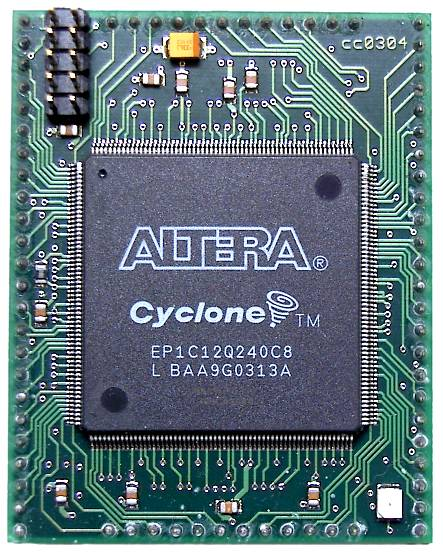
\includegraphics[height=64mm]{appendix/cycore_top}
    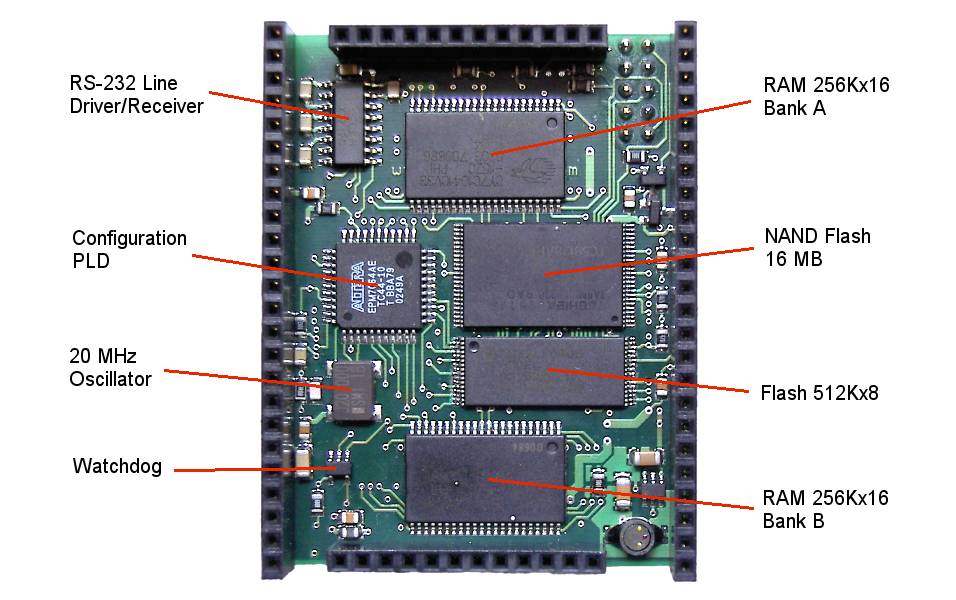
\includegraphics[height=67mm]{appendix/cycore_bottom}
    \caption{Top and bottom side of the Cyclone FPGA board}
\end{figure}
\begin{figure}
    \centering
    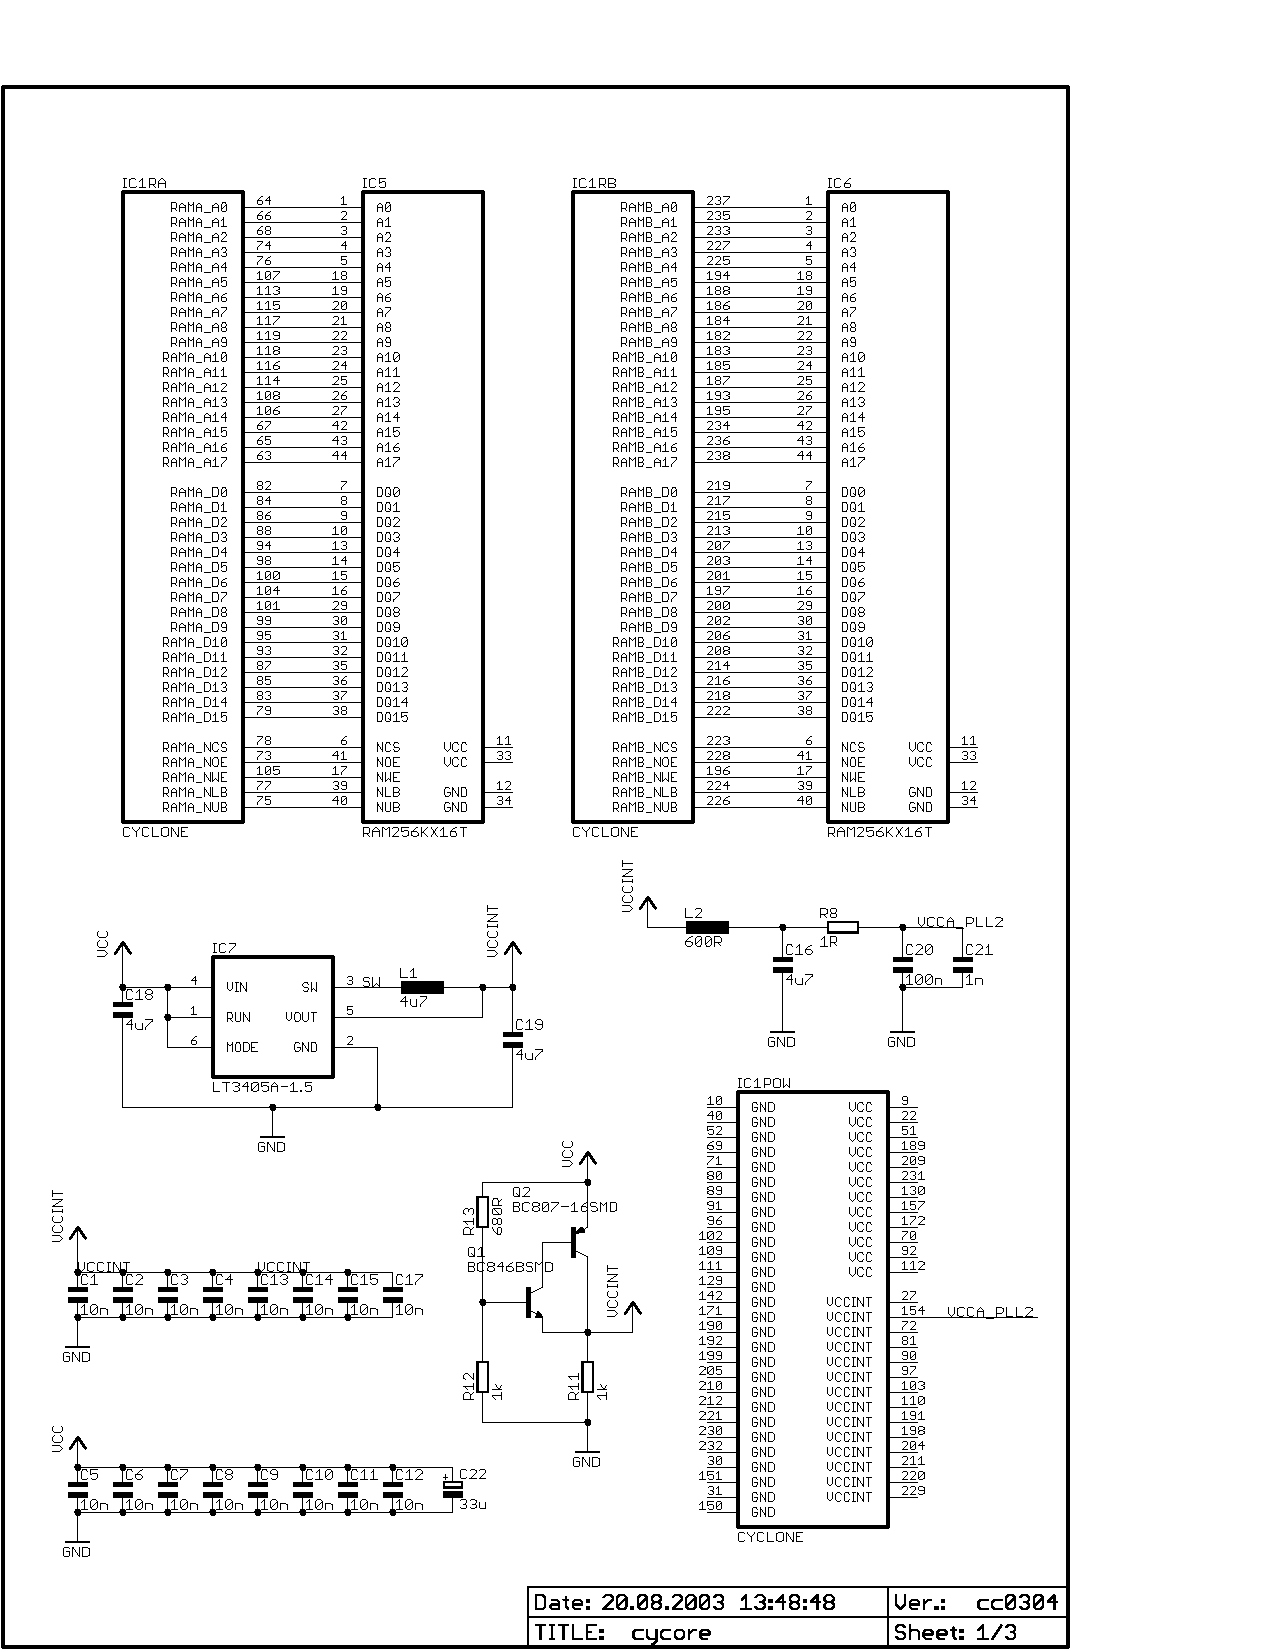
\includegraphics[scale=0.87]{appendix/cycore_p1}
    \caption{Schematic of the Cyclone FPGA board, page 1}
\end{figure}
\begin{figure}
    \centering
    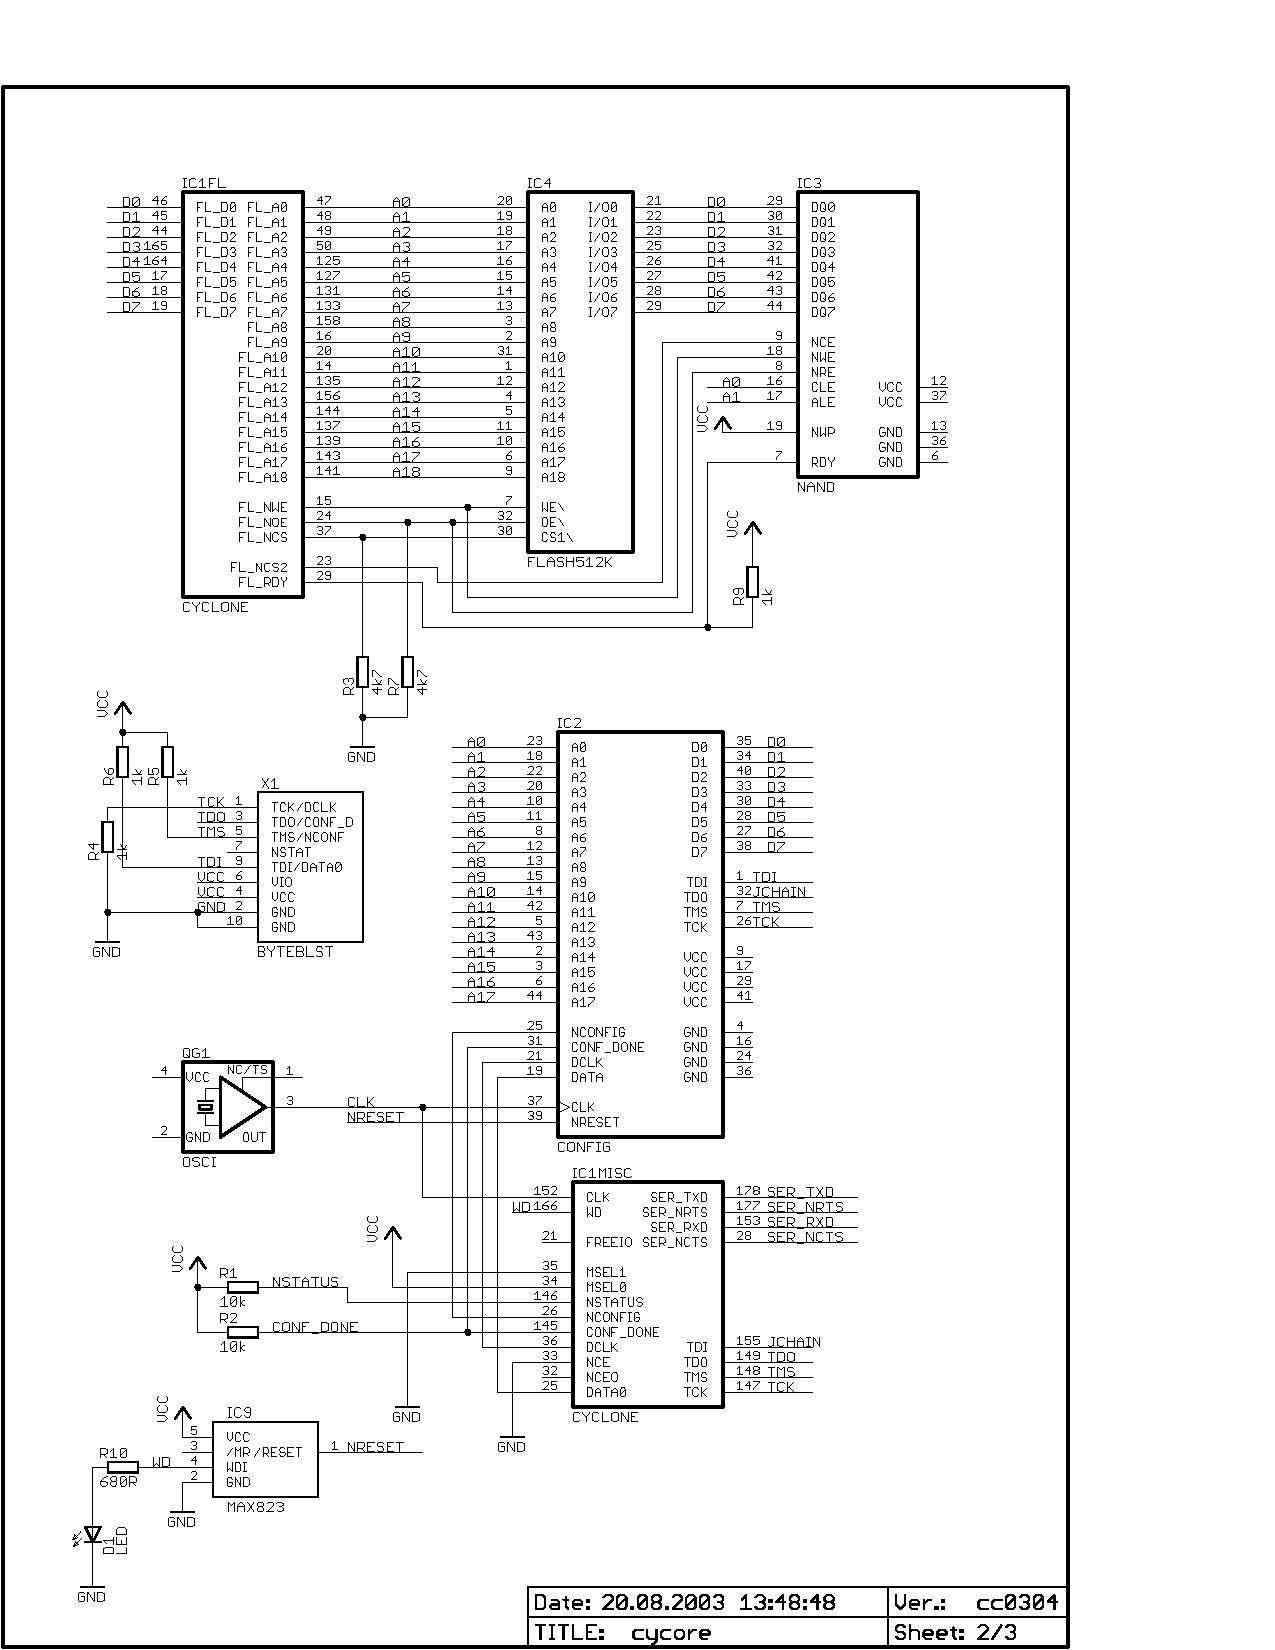
\includegraphics[scale=0.87]{appendix/cycore_p2}
    \caption{Schematic of the Cyclone FPGA board, page 2}
\end{figure}
\begin{figure}
    \centering
    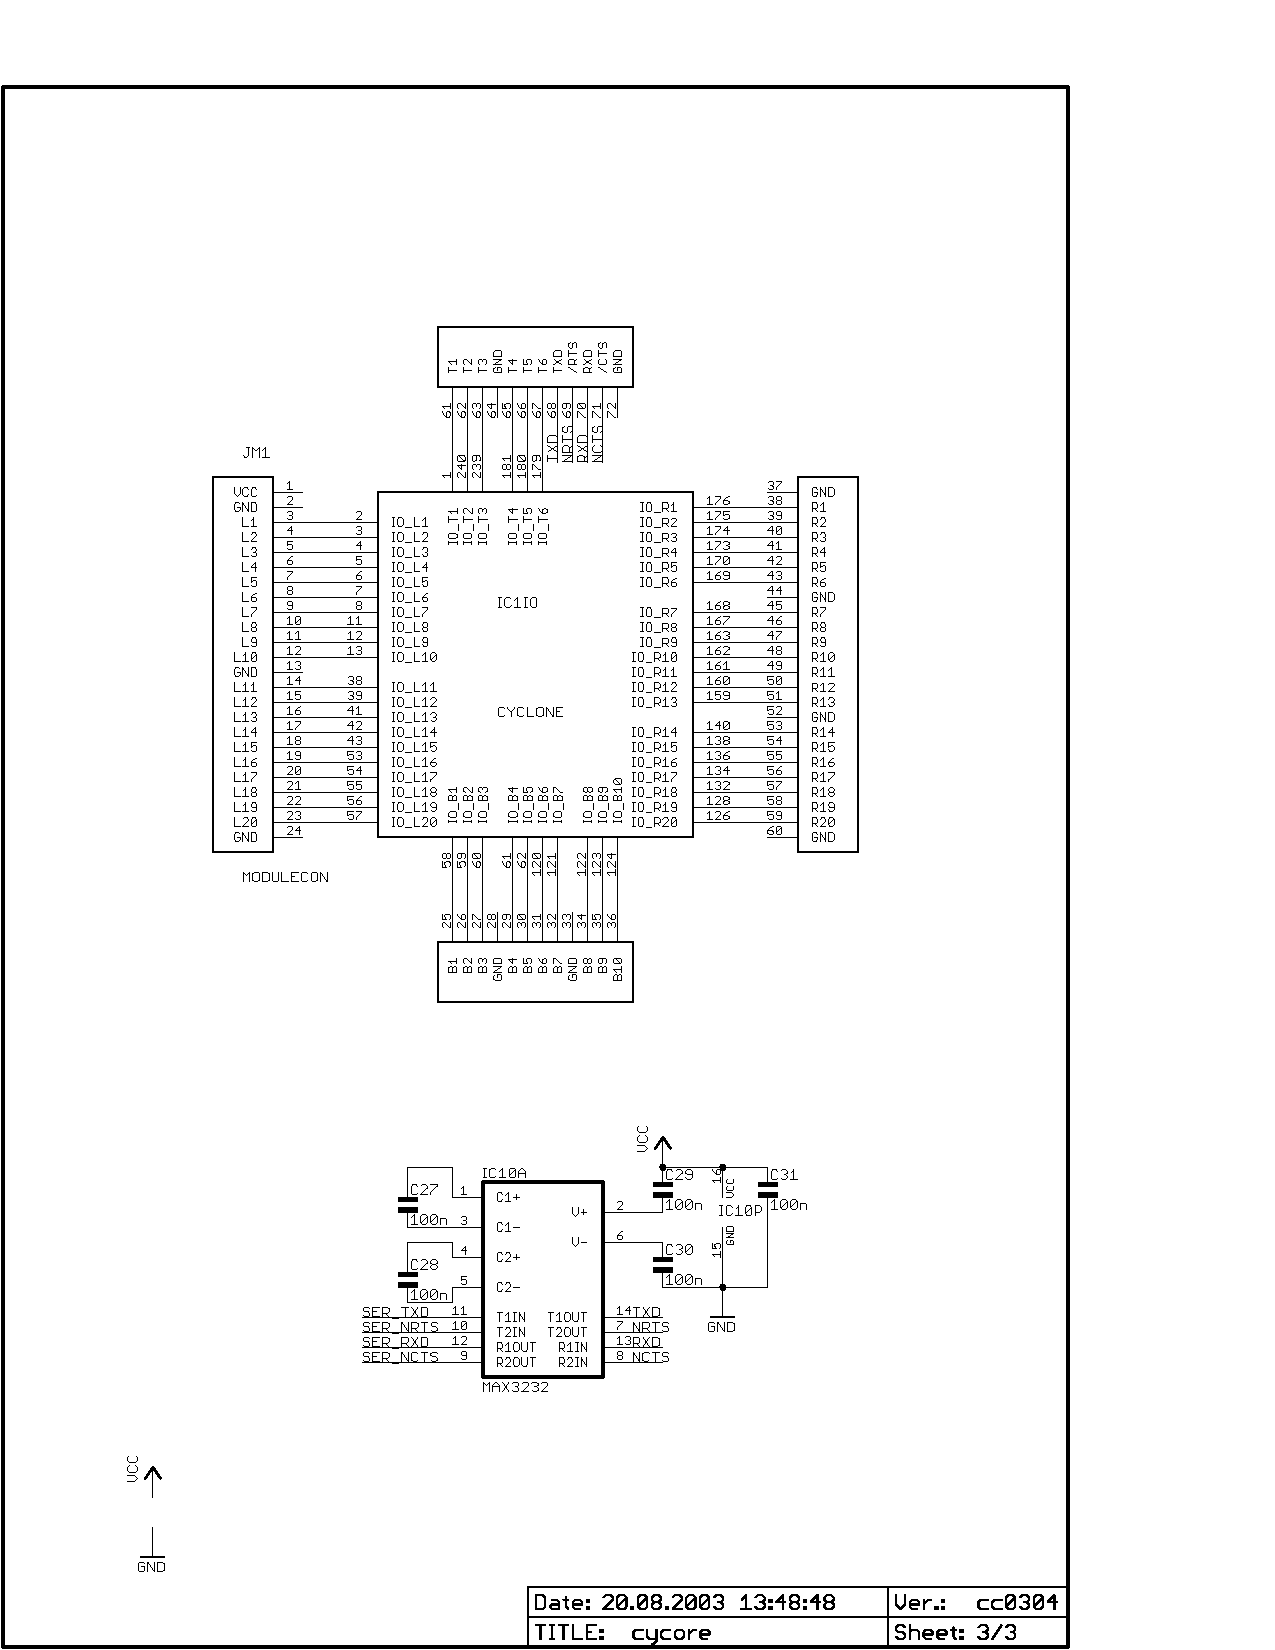
\includegraphics[scale=0.87]{appendix/cycore_p3}
    \caption{Schematic of the Cyclone FPGA board, page 3}
\end{figure}



\end{document}
